        %%******************************************%%
        %%                                          %%
        %%        Modello di tesi di laurea         %%
        %%            di Andrea Giraldin            %%
        %%                                          %%
        %%             2 novembre 2012              %%
        %%                                          %%
        %%******************************************%%


% I seguenti commenti speciali impostano:
% 1. 
% 2. PDFLaTeX come motore di composizione;
% 3. tesi.tex come documento principale;
% 4. il controllo ortografico italiano per l'editor.

% !TEX encoding = UTF-8
% !TEX TS-program = pdflatex
% !TEX root = tesi.tex
% !TEX spellcheck = it-IT

\documentclass[10pt,                    % corpo del font principale
               a4paper,                 % carta A4
               twoside,                 % impagina per fronte-retro
               openright,               % inizio capitoli a destra
               english,                 
               italian,                 
               ]{book}    

\usepackage[utf8]{inputenc}             % codifica di input; anche [latin1] va bene
                                        % NOTA BENE! va accordata con le preferenze dell'editor

%**************************************************************
% Importazione package
%************************************************************** 

%\usepackage{amsmath,amssymb,amsthm}    % matematica

\usepackage[english, italian]{babel}    % per scrivere in italiano e in inglese;
                                        % l'ultima lingua (l'italiano) risulta predefinita

\usepackage{bookmark}                   % segnalibri

\usepackage{caption}                    % didascalie

\usepackage{chngpage,calc}              % centra il frontespizio

\usepackage{csquotes}                   % gestisce automaticamente i caratteri (")

\usepackage{emptypage}                  % pagine vuote senza testatina e piede di pagina

\usepackage{epigraph}					% per epigrafi

\usepackage{enumitem}					% per liste strette

\usepackage{eurosym}                    % simbolo dell'euro

\usepackage[T1]{fontenc}                % codifica dei font:
                                        % NOTA BENE! richiede una distribuzione *completa* di LaTeX

%\usepackage{indentfirst}               % rientra il primo paragrafo di ogni sezione

\usepackage{graphicx}                   % immagini

\usepackage{hyperref}                   % collegamenti ipertestuali



\usepackage[binding=5mm]{layaureo}      % margini ottimizzati per l'A4; rilegatura di 5 mm

\usepackage{listings}                   % codici

\usepackage{microtype}                  % microtipografia

\usepackage{mparhack,fixltx2e,relsize}  % finezze tipografiche

\usepackage{nameref}                    % visualizza nome dei riferimenti                                      

\usepackage[font=small]{quoting}        % citazioni

\usepackage{subfig}                     % sottofigure, sottotabelle

\usepackage[italian]{varioref}          % riferimenti completi della pagina

\usepackage[dvipsnames]{xcolor}         % colori

\usepackage{booktabs}                   % tabelle                                       
\usepackage{tabularx}                   % tabelle di larghezza prefissata                                    
\usepackage{longtable}                  % tabelle su più pagine                                        
\usepackage{ltxtable}                   % tabelle su più pagine e adattabili in larghezza

\usepackage[toc, acronym]{glossaries}   % glossario
                                        % per includerlo nel documento bisogna:
                                        % 1. compilare una prima volta tesi.tex;
                                        % 2. eseguire: makeindex -s tesi.ist -t tesi.glg -o tesi.gls tesi.glo
                                        % 3. eseguire: makeindex -s tesi.ist -t tesi.alg -o tesi.acr tesi.acn
                                        % 4. compilare due volte tesi.tex.

\usepackage[backend=biber,style=verbose-ibid,hyperref,backref]{biblatex}
                                        % eccellente pacchetto per la bibliografia; 
                                        % produce uno stile di citazione autore-anno; 
                                        % lo stile "numeric-comp" produce riferimenti numerici
                                        % per includerlo nel documento bisogna:
                                        % 1. compilare una prima volta tesi.tex;
                                        % 2. eseguire: biber tesi
                                        % 3. compilare ancora tesi.tex.

%**************************************************************
% file contenente le impostazioni della tesi
%**************************************************************

%**************************************************************
% Frontespizio
%**************************************************************
\newcommand{\myName}{Davide Bortot}                             % autore
\newcommand{\myTitle}{Project Tango e PCL: un'applicazione pratica alle 'Nuvole di Punti'}                    	% titolo tesi
\newcommand{\myDegree}{Tesi di laurea triennale}                % tipo di tesi
\newcommand{\myUni}{Università degli Studi di Padova}           % università
\newcommand{\myFaculty}{Corso di Laurea in Informatica}         % facoltà
\newcommand{\myDepartment}{Dipartimento di Matematica}          % dipartimento
\newcommand{\myProf}{Ombretta Gaggi}                            % relatore
\newcommand{\myLocation}{Padova}                                % dove
\newcommand{\myAA}{2015-2016}                                   % anno accademico
\newcommand{\myTime}{Oct 2016}                                  % quando


%**************************************************************
% Impostazioni di impaginazione
% see: http://wwwcdf.pd.infn.it/AppuntiLinux/a2547.htm
%**************************************************************

\setlength{\parindent}{14pt}   % larghezza rientro della prima riga
\setlength{\parskip}{0pt}   % distanza tra i paragrafi


%**************************************************************
% Impostazioni di biblatex
%**************************************************************
\bibliography{bibliografia} % database di biblatex 

\defbibheading{bibliography}
{
    \cleardoublepage
    \phantomsection 
    \addcontentsline{toc}{chapter}{\bibname}
    \chapter*{\bibname\markboth{\bibname}{\bibname}}
}

\setlength\bibitemsep{1.5\itemsep} % spazio tra entry

\DeclareBibliographyCategory{opere}
\DeclareBibliographyCategory{web}

\addtocategory{opere}{womak:lean-thinking}
\addtocategory{web}{site:agile-manifesto}

\defbibheading{opere}{\section*{Riferimenti bibliografici}}
\defbibheading{web}{\section*{Siti Web consultati}}


%**************************************************************
% Impostazioni di caption
%**************************************************************
\captionsetup{
    tableposition=top,
    figureposition=bottom,
    font=small,
    format=hang,
    labelfont=bf
}

%**************************************************************
% Impostazioni di glossaries
%**************************************************************

%**************************************************************
% Acronimi
%**************************************************************
\renewcommand{\acronymname}{Acronimi e abbreviazioni}

\newacronym[description={\glslink{apig}{Application Program Interface}}]
    {api}{API}{Application Program Interface}

\newacronym[description={\glslink{umlg}{Unified Modeling Language}}]
    {uml}{UML}{Unified Modeling Language}
       
\newacronym[description={\glslink{PCL}{Point Cloud Library}}]
    {pcl}{PCL}{Point Cloud Library}     

%**************************************************************
% Glossario
%**************************************************************
%\renewcommand{\glossaryname}{Glossario}

\newglossaryentry{PCL}
{
    name=\glslink{PCL}{PCL},
    text=PCL,
    sort=PCL,
    description={Una  delle librerie di maggior rilievo nel campo della \emph{Computer Vision}, \emph{Open Source}, scritta in C++, di algoritmi per l'elaborazione di \emph{Point Cloud} tridimensionali. Contiene algoritmi per il filtraggio, la segmentazione, la \emph{registration} e il \emph{meshing} di Point Cloud, per citarne alcuni. \\
La libreria è ampiamente utilizzata da qualsiasi applicativo debba trattare nuvole di punti, ed oltre ad essere utile ed efficiente è anche ben documentata, con molti esempi d'utilizzo reperibili online.\\
Le notevoli potenzialità della libreria sono state utilizzate intensivamente nell'applicativo con lo scopo di isolare i punti appartenenti all'oggetto scansionato dal resto del Point Cloud, ed effettuarne quindi il meshing.}
}

\newglossaryentry{umlg}
{
    name=\glslink{uml}{UML},
    text=UML,
    sort=uml,
    description={in ingegneria del software \emph{UML, Unified Modeling Language} (ing. linguaggio di modellazione unificato) è un linguaggio di modellazione e specifica basato sul paradigma object-oriented. L'\emph{UML} svolge un'importantissima funzione di ``lingua franca'' nella comunità della progettazione e programmazione a oggetti. Gran parte della letteratura di settore usa tale linguaggio per descrivere soluzioni analitiche e progettuali in modo sintetico e comprensibile a un vasto pubblico}
}

\newglossaryentry{Point Cloud} {
	name = \glslink{Point Cloud}{Point Cloud},
	text = Point Cloud,
	sort = Point Cloud,
	description = {Un \emph{Point Cloud} è modello matematico che descrive un oggetto tridimensionale semplicemente come insieme del maggior numero possibile di punti dell'oggetto stesso.\\
È molto usato in ambito di \emph{Computer vision} e realtà aumentata}
}


\newglossaryentry{API} {
	name = \glslink{API}{API},
	text = API,
	sort = API,
	description = {Con \emph{API} o \emph{Application Programming Interface} si intende ogni insieme di metodi e procedure resi disponibili al programmatore. Di solito raggruppati a formare un set di strumenti specifici per l'esecuzione di un determinato compito}
}

\newglossaryentry{artefatto} {
	name = \glslink{artefatto}{Artefatto},
	text = artefatto,
	plural = artefatti,
	sort = artefatto,
	description = {Gli \emph{artefatti} sono degli elementi presenti all'interno di una ricostruzione \emph{Point Cloud} ma non nella realtà, dovuti errori nella rilevazione. Sono generalmente di forma planare e sospesi qualche centimetro al di sopra del pavimento}
}

\newglossaryentry{Design Pattern} {
	name = \glslink{Design Pattern}{Design Pattern},
	text = Design Pattern,
	sort = design pattern,
	description = {Un \emph{Design Pattern} è una soluzione progettuale di comprovata bontà ad un problema ricorrente in un certo contesto}
}

\newglossaryentry{ghosting} {
	name = \glslink{ghosting}{Ghosting},
	text = ghosting,
	sort = ghosting,
	description = {Il problema del \emph{Ghosting} affligge alcune registrazioni effettuate con il prodotto: è dovuto ad una errata stima della posizione del dispositivo e produce ricostruzioni tridimensionali affette da errori. Se visualizzate graficamente il tali ricostruzioni presentano l'oggetto come se fosse sdoppiato, ad esempio come in figura \ref{fig:no_drift_correction}}
}

\newglossaryentry{feature} {
	name = \glslink{feature}{Feature},
	text = feature,
	sort = feature,
	description = {Una \emph{feature} è un punto particolare nello spazio che il processo di \emph{Area Learning} ritiene facilmente riconoscibile, e che quindi è salvato ed usato come punto di riferimento in un determinato ambiente. Un'area ha generalmente qualche centinaio di \emph{feature}}
}

\newglossaryentry{Fisheye} {
	name = \glslink{Fisheye}{Fotocamera Fisheye},
	text = fotocamera Fisheye,
	sort = Fotocamera Fisheye,
	description = {Una Fotocamera \emph{Fish-eye} dispone di un obiettivo grandangolare che abbraccia un angolo di campo di circa 180 gradi, in particolare quella in dotazione nel dispositivo usato è in bianco e nero}
}	

\newglossaryentry{mesh} {
	name = \glslink{mesh}{Mesh},
	text = mesh,
	plural = meshes,
	sort = Mesh,
	description = {Una \emph{mesh} o \emph{mesh} poligonale è una collezione di vertici, spigoli e facce che definiscono la forma di un oggetto tridimensionale}
}	

\newglossaryentry{Motion Tracking} {
	name = \glslink{Motion Tracking}{Motion Tracking},
	text = Motion Tracking,
	sort = Motion Tracking,
	description = {Il \emph{Motion Tracking} è una tecnica che permette al dispositivo di tracciare i suoi movimenti all'interno di un area}
}	

\newglossaryentry{drifting} {
	name = \glslink{drifting}{Drifting},
	text = drifting,
	sort = Drifting,
	description = {Il \emph{drifting} è l'errore di calcolo nella posizione di un dispositivo che utilizza il \emph{Motion Tracking}, che ne causa una scorretta stima della posizione.}
}	

\newglossaryentry{Project Tango} {
	name = \glslink{Project Tango}{Project Tango},
	text = Project Tango,
	sort = Project Tango,
	description = {Il progetto \emph{Tango} è un progetto promosso e portato avanti da \emph{Google}. Si propone di promuovere nuovi tipi di dispositivi dotati di \emph{Hardware} innovativo, come fotocamera \emph{Fish-Eye}, sensore di profondità etc. Grazie ai loro sensori i dispositivi \emph{Tango} sono in grado di avere una certa conoscenza dell'ambiente che li circonda: sono in grado di tracciare il proprio movimento ed orientazione, di ricordare gli ambienti dove sono già stati, di avere una visione tridimensionale degli oggetti}
}	
%
\newglossaryentry{voxel} {
	name = \glslink{voxel}{Voxel},
	text = voxel,
	sort = Voxel,
	description = {Un \emph{voxel}, detto anche \emph{pixel} volumetrico, è un elemento di volume che rappresenta un valore di intensità di segnale o di colore in uno spazio tridimensionale}
}	
%




 % database di termini
\makeglossaries


%**************************************************************
% Impostazioni di graphicx
%**************************************************************
\graphicspath{{immagini/}} % cartella dove sono riposte le immagini


%**************************************************************
% Impostazioni di hyperref
%**************************************************************
\hypersetup{
    %hyperfootnotes=false,
    %pdfpagelabels,
    %draft,	% = elimina tutti i link (utile per stampe in bianco e nero)
    colorlinks=true,
    linktocpage=true,
    pdfstartpage=1,
    pdfstartview=FitV,
    % decommenta la riga seguente per avere link in nero (per esempio per la stampa in bianco e nero)
    %colorlinks=false, linktocpage=false, pdfborder={0 0 0}, pdfstartpage=1, pdfstartview=FitV,
    breaklinks=true,
    pdfpagemode=UseNone,
    pageanchor=true,
    pdfpagemode=UseOutlines,
    plainpages=false,
    bookmarksnumbered,
    bookmarksopen=true,
    bookmarksopenlevel=1,
    hypertexnames=true,
    pdfhighlight=/O,
    %nesting=true,
    %frenchlinks,
    urlcolor=webbrown,
    linkcolor=RoyalBlue,
    citecolor=webgreen,
    %pagecolor=RoyalBlue,
    %urlcolor=Black, linkcolor=Black, citecolor=Black, %pagecolor=Black,
    pdftitle={\myTitle},
    pdfauthor={\textcopyright\ \myName, \myUni, \myFaculty},
    pdfsubject={},
    pdfkeywords={},
    pdfcreator={pdfLaTeX},
    pdfproducer={LaTeX}
}

%**************************************************************
% Impostazioni di itemize
%**************************************************************
\renewcommand{\labelitemi}{$\ast$}

%\renewcommand{\labelitemi}{$\bullet$}
%\renewcommand{\labelitemii}{$\cdot$}
%\renewcommand{\labelitemiii}{$\diamond$}
%\renewcommand{\labelitemiv}{$\ast$}


%**************************************************************
% Impostazioni di listings
%**************************************************************
\lstset{
    language=[LaTeX]Tex,%C++,
    keywordstyle=\color{RoyalBlue}, %\bfseries,
    basicstyle=\small\ttfamily,
    %identifierstyle=\color{NavyBlue},
    commentstyle=\color{Green}\ttfamily,
    stringstyle=\rmfamily,
    numbers=none, %left,%
    numberstyle=\scriptsize, %\tiny
    stepnumber=5,
    numbersep=8pt,
    showstringspaces=false,
    breaklines=true,
    frameround=ftff,
    frame=single
} 


%**************************************************************
% Impostazioni di xcolor
%**************************************************************
\definecolor{webgreen}{rgb}{0,.5,0}
\definecolor{webbrown}{rgb}{.6,0,0}


%**************************************************************
% Altro
%**************************************************************

\newcommand{\omissis}{[\dots\negthinspace]} % produce [...]

% eccezioni all'algoritmo di sillabazione
\hyphenation
{
    ma-cro-istru-zio-ne
    gi-ral-din
}

\newcommand{\sectionname}{sezione}
\addto\captionsitalian{\renewcommand{\figurename}{figura}
                       \renewcommand{\tablename}{tabella}}

\newcommand{\glsfirstoccur}{\ap{{[g]}}}

\newcommand{\intro}[1]{\emph{\textsf{#1}}}

%**************************************************************
% Environment per ``rischi''
%**************************************************************
\newcounter{riskcounter}                % define a counter
\setcounter{riskcounter}{0}             % set the counter to some initial value

%%%% Parameters
% #1: Title
\newenvironment{risk}[1]{
    \refstepcounter{riskcounter}        % increment counter
    \par \noindent                      % start new paragraph
    \textbf{\arabic{riskcounter}. #1}   % display the title before the 
                                        % content of the environment is displayed 
}{
    \par\medskip
}

\newcommand{\riskname}{Rischio}

\newcommand{\riskprob}[1]{\textbf{\\Probabilità:} #1.}

\newcommand{\riskimpact}[1]{\textbf{\\Impatto:} #1.}

\newcommand{\riskdescription}[1]{\textbf{\\Descrizione:} #1.}

\newcommand{\risksolution}[1]{\textbf{\\Gestione:} #1.}

%**************************************************************
% Environment per ``use case''
%**************************************************************
\newcounter{usecasecounter}             % define a counter
\setcounter{usecasecounter}{0}          % set the counter to some initial value

%%%% Parameters
% #1: ID
% #2: Nome
\newenvironment{usecase}[2]{
    \renewcommand{\theusecasecounter}{\usecasename #1}  % this is where the display of 
                                                        % the counter is overwritten/modified
    \refstepcounter{usecasecounter}             % increment counter
    \vspace{10pt}
    \par \noindent                              % start new paragraph
    {\large \textbf{\usecasename #1: #2}}       % display the title before the 
                                                % content of the environment is displayed 
    \medskip
}{
    \medskip
}

\newcommand{\usecasename}{UC}

\newcommand{\usecaseactors}[1]{\textbf{\\Attori Principali:} #1. \vspace{4pt}}
\newcommand{\usecasepre}[1]{\textbf{\\Precondizioni:} #1. \vspace{4pt}}
\newcommand{\usecasedesc}[1]{\textbf{\\Descrizione:} #1. \vspace{4pt}}
\newcommand{\usecasepost}[1]{\textbf{\\Postcondizioni:} #1. \vspace{4pt}}
\newcommand{\usecasealt}[1]{\textbf{\\Scenario Alternativo:} #1. \vspace{4pt}}

%**************************************************************
% Environment per ``namespace description''
%**************************************************************

\newenvironment{namespacedesc}{
    \vspace{10pt}
    \par \noindent                              % start new paragraph
    \begin{description} 
}{
    \end{description}
    \medskip
}

\newcommand{\classdesc}[2]{\item[\textbf{#1:}] #2}                     % file con le impostazioni personali

\begin{document}
%**************************************************************
% Materiale iniziale
%**************************************************************
\frontmatter
% !TEX encoding = UTF-8
% !TEX TS-program = pdflatex
% !TEX root = ../tesi.tex
% !TEX spellcheck = it-IT

%**************************************************************
% Frontespizio 
%**************************************************************
\begin{titlepage}

\begin{center}

\begin{LARGE}
\textbf{\myUni}\\
\end{LARGE}

\vspace{10pt}

\begin{Large}
\textsc{\myDepartment}\\
\end{Large}

\vspace{10pt}

\begin{large}
\textsc{\myFaculty}\\
\end{large}

\vspace{30pt}
\begin{figure}[htbp]
\begin{center}

\includegraphics[height=6cm]{logo-unipd}
\end{center}
\end{figure}
\vspace{30pt} 

\begin{LARGE}
\begin{center}
\textbf{\myTitle}\\
\end{center}
\end{LARGE}

\vspace{10pt} 

\begin{large}
\textsl{\myDegree}\\
\end{large}

\vspace{40pt} 

\begin{large}
\begin{flushleft}
\textit{Relatore}\\ 
\vspace{5pt} 
Prof. \myProf
\end{flushleft}

\vspace{0pt} 

\begin{flushright}
\textit{Laureando}\\ 
\vspace{5pt} 
\myName \\
\vspace{2pt} 
\myID
\end{flushright}
\end{large}

\vspace{25pt}	%was 40

\line(1, 0){338} \\
\begin{normalsize}
\textsc{Anno Accademico \myAA}
\end{normalsize}

\end{center}
\end{titlepage} 
% !TEX encoding = UTF-8
% !TEX TS-program = pdflatex
% !TEX root = ../tesi.tex
% !TEX spellcheck = it-IT

%**************************************************************
% Colophon
%**************************************************************
\clearpage
\phantomsection
\thispagestyle{empty}

\hfill

\vfill

\noindent\myName: \textit{\myTitle,}
\myDegree,
\textcopyright\ \myTime.
%% !TEX encoding = UTF-8
% !TEX TS-program = pdflatex
% !TEX root = ../tesi.tex
% !TEX spellcheck = it-IT

%**************************************************************
% Dedica
%**************************************************************
\cleardoublepage
\phantomsection
\thispagestyle{empty}
\pdfbookmark{Dedica}{Dedica}

\vspace*{3cm}

\begin{center}
Lorem ipsum dolor sit amet, consectetuer adipiscing elit. \\ \medskip
--- Oscar Wilde    
\end{center}

\medskip

\begin{center}
Dedicato a ...
\end{center}

% !TEX encoding = UTF-8
% !TEX TS-program = pdflatex
% !TEX root = ../tesi.tex
% !TEX spellcheck = it-IT

%**************************************************************
% Sommario
%**************************************************************
\cleardoublepage
\phantomsection
\pdfbookmark{Sommario}{Sommario}
\begingroup
\let\clearpage\relax
\let\cleardoublepage\relax
\let\cleardoublepage\relax

\chapter*{Sommario}

Il presente documento descrive il lavoro svolto durante il periodo di stage, della durata di circa trecentoventi ore, dal laureando Davide Bortot presso l'azienda VIC S.r.l.
Obbiettivo del tirocinio era lo sviluppo di un'applicazione prototipale per il \emph{tablet Project Tango} per l'aquisizione di scansioni di oggetti reali sotto forma di 'Nuvola di Punti'. \\
In primo luogo era richiesto il filtraggio e l'elaborazione dei dati acquisiti in modo da isolare l'oggetto scansionato, e successivamente di creare una \emph{mesh} tridimensionale a partire dai punti rimanenti. Scopo finale era calcolare il volume dell'oggetto tridimensionale così ottenuto.

%\vfill
%
%\selectlanguage{english}
%\pdfbookmark{Abstract}{Abstract}
%\chapter*{Abstract}
%
%\selectlanguage{italian}

\endgroup			

\vfill


% !TEX encoding = UTF-8
% !TEX TS-program = pdflatex
% !TEX root = ../tesi.tex
% !TEX spellcheck = it-IT

%**************************************************************
% Ringraziamenti
%**************************************************************
\cleardoublepage
\phantomsection
\pdfbookmark{Ringraziamenti}{ringraziamenti}

\begin{flushright}{
	\slshape    
	``Life is really simple, but we insist on making it complicated''} \\ 
	\medskip
    --- Confucius
\end{flushright}


\bigskip

\begingroup
\let\clearpage\relax
\let\cleardoublepage\relax
\let\cleardoublepage\relax

\chapter*{Ringraziamenti}

\noindent \textit{Innanzitutto, vorrei esprimere la mia gratitudine alla Prof.ssa Ombretta Gaggi, relatore della mia tesi, per l'aiuto e il sostegno fornitomi durante la stesura del lavoro.}\\

\noindent \textit{In secondo luogo, ringrazio Michele Marchetto, tutor aziendale, così come tutti i colleghi Tommaso Padovan, Lorenzo Ceccon e Luca D'Ambros per aver reso lo stage un'esperienza di crescita.}\\

\noindent \textit{Ringrazio col cuore i miei genitori Giulia e Carlo per aver creduto in me in ogni momento e avermi sempre sostenuto.}\\

\noindent \textit{Infine ringrazio i miei amici di sempre e gli amici nuovi che ho incontrato nel mio percorso universitario, per avermi reso quello che sono.}\\
\bigskip

\noindent\textit{\myLocation, \myTime}
\hfill \myName

\endgroup


% !TEX encoding = UTF-8
% !TEX TS-program = pdflatex
% !TEX root = ../tesi.tex
% !TEX spellcheck = it-IT

%**************************************************************
% Indici
%**************************************************************
\cleardoublepage
\pdfbookmark{\contentsname}{tableofcontents}
\setcounter{tocdepth}{2}
\tableofcontents
%\markboth{\contentsname}{\contentsname} 
\clearpage

\begingroup 
    \let\clearpage\relax
    \let\cleardoublepage\relax
    \let\cleardoublepage\relax
    %*******************************************************
    % Elenco delle figure
    %*******************************************************    
    \phantomsection
    \pdfbookmark{\listfigurename}{lof}
    \listoffigures

    \vspace*{8ex}

    %*******************************************************
    % Elenco delle tabelle
    %*******************************************************
    \phantomsection
    \pdfbookmark{\listtablename}{lot}
    \listoftables
        
    \vspace*{8ex}
\endgroup

\cleardoublepage

\cleardoublepage

%**************************************************************
% Materiale principale
%**************************************************************
\mainmatter
% !TEX encoding = UTF-8
% !TEX TS-program = pdflatex
% !TEX root = ../tesi.tex
% !TEX spellcheck = it-IT

%**************************************************************
\chapter{Introduzione}
\label{cap:introduzione}
%**************************************************************

%Introduzione al contesto applicativo.\\

%\noindent Esempio di utilizzo di un termine nel glossario \\
%\gls{api}. \\

%\noindent Esempio di citazione in linea \\
%\cite{site:agile-manifesto}. \\

%\noindent Esempio di citazione nel pie' di pagina \\
%citazione\footcite{womak:lean-thinking} \\

%**************************************************************
\section{L'azienda}

VIC è stata fondata da Alessio Bisutti che, dopo aver sviluppato una lunga esperienza
nel campo ispettivo, ha deciso di costituire una società in grado di offrire ai propri clienti un servizio professionale, chiaro ed affidabile, appoggiandosi alle nuove tecnologie.
Si occupa di controlli per grandi ordini, sia di materie prime che di semi-lavorati, di
cui individua e riporta eventuali danni, carenze nella spedizione e non conformità con
quanto ordinato.
VIC viene fondata a Venezia 7 anni fa come piccola società di ispezione locale. Fin dall'inizio, l'obiettivo principale di VIC è stato la riduzione del tempo tra ispezione e reporting al cliente. Ora l'obiettivo è raggiunto, perchè VIC sta fornendo ai suoi clienti tutti i risultati e le informazioni importanti in tempo reale, senza alcun ritardo, grazie agli investimenti fatti nel campo della tecnologia e delle applicazioni mobili.

%**************************************************************
\section{L'idea}

I più importanti obbiettivi del controllo qualità effettuato durante un ispezione sono il determinare la corretta forma, peso, quantità e dimensioni degli oggetti da esaminare.\\
Gli ispettori possono scattare fotografie, prendere appunti e sfruttare la loro esperienza per fornire stime accurate; si è manifestata però la necessità di affiancare queste ultime a dei dati quanto più possibile oggettivi e rapidi da ottenere.\\
Da qui nasce l'idea di fornire agli ispettori uno strumento informatico in grado di effettuare queste stime. Grazie alla ricostruzione computerizzata resa disponibile dai \emph{Tango device} sarà possibile non solo visualizzare su uno schermo il modello 3D del soggetto della ispezione, ma anche ottenere ulteriori dati utili quali:
\begin{itemize}
	\item Una stima del volume, e se necessario del peso, dell'oggetto.
	\item L'esito del confronto dell'oggetto con un modello ideale, per evidenziare eventuali danni o deformazioni.
\end{itemize}
Con il prototipo realizzato durante lo \emph{stage} sono rese disponibili solamente le funzionalità di ricostruzione dell'oggetto e calcolo (approssimato) del volume.\\
Le operazioni troppo computazionalmente costose da effettuare su tablet, quali il filtraggio e \emph{meshing} dei punti acquisiti, sono state delegate ad un \emph{backend server} che effettui le elaborazioni necessarie ed invii i risultati al richiedente, mentre all'applicativo per tablet è stato affidato il compito di aquisire e visualizzare un oggetto sotto forma di 'Nuvola di Punti' e poterne esaminare la \emph{mesh} ottenuta.

%**************************************************************
\section{Cos'è Project Tango}

Project Tango è un \emph{tablet} sperimentale prodotto da \emph{Google} in grado di scandire tridimensionalmente l'ambiente circostante e di tracciare la propria posizione rispetto ad esso. Ciò è possibile attraverso il ricco hardware di cui è dotato (si veda la figura \ref{fig:tango_hardware}), tra cui:
\begin{itemize}
\item una fotocamera RBG-IR\\
\item una fotocamera \emph{Fisheye}\\
\item un sensore di profondità IR\\
\item accelerometro e giroscopio\\
\end{itemize}

\begin{figure}[!h] 
    \centering 
    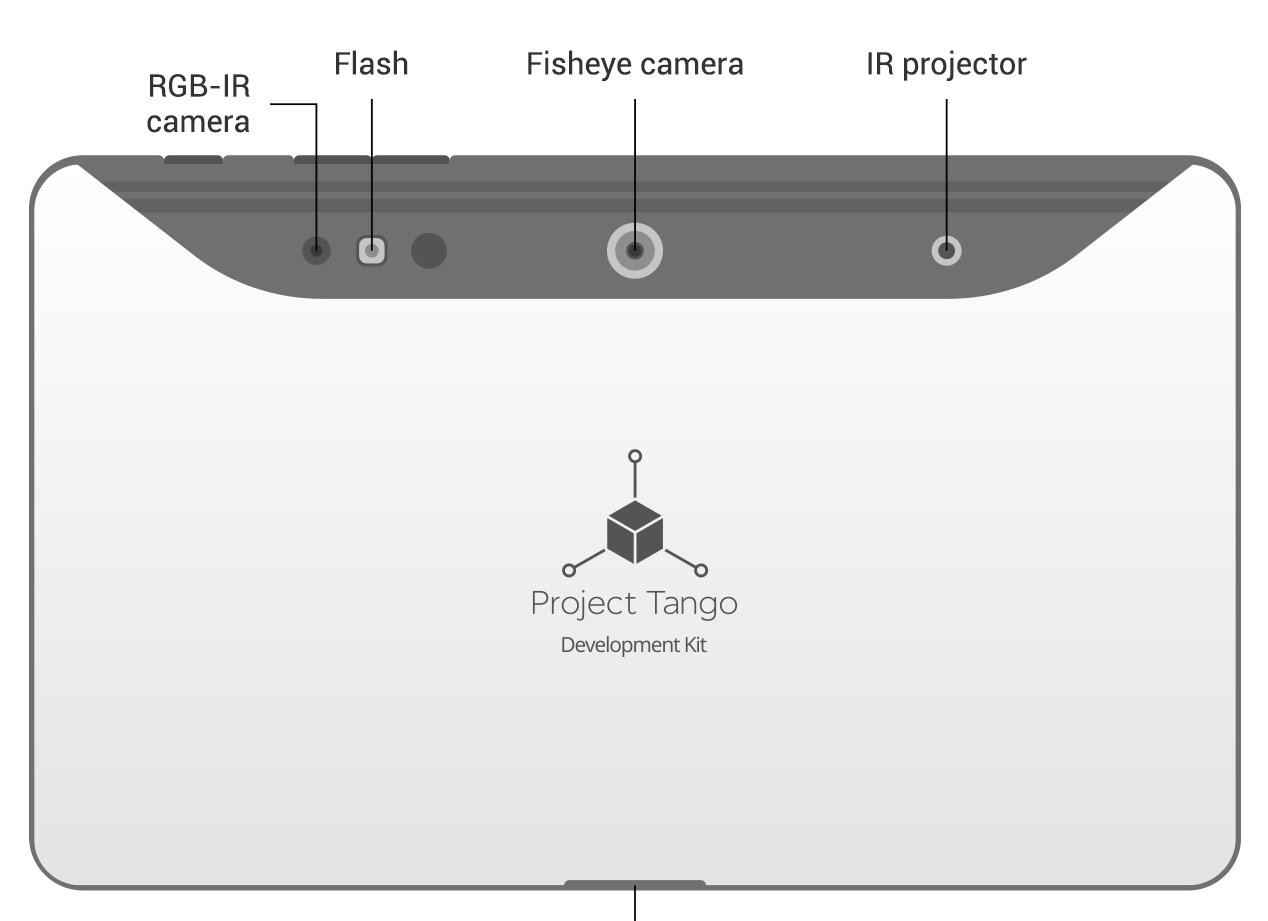
\includegraphics[width=0.9\columnwidth]{varie/tango-hardware.png} 
    \caption{L' \emph{hardware} di \emph{Project Tango}}
    \label{fig:tango_hardware}
\end{figure}

\noindent
Project Tango è quindi specificamente pensato per sviluppare applicazioni che necessitano di comprendere ed estrapolare informazioni dal mondo reale (ad es. realtà aumentata).
Le funzionalità del \emph{tablet} sono accessibili attraverso le \emph{Tango API}, le \emph{API} ufficiali per lo sviluppo di applicazioni \emph{Tango}.

%**************************************************************
\section{Lavoro svolto}
Al tirocinante è stato richiesto di focalizzarsi sullo sviluppo del lato server dell'applicazione, in modo che fosse possibile ricevere ed elaborare 'Nuvole di Punti', ed ottenere i risultati elaborati, lavorando nel mentre in stretta collaborazione con un altro stagista, Tommaso Padovan (laureando il 13 Ottobre, relatore il Prof. Gilberto Filè) che si occupava dell'applicazione lato client. Nell'ultimo periodo di stage la parte server era già a buon punto, quindi il focus del tirocinio si è spostato sul miglioramento dell'applicativo lato client.

%**************************************************************
\section{Il Prodotto - lato client}

L'applicazione su \emph{tablet} prodotta realizza, seppur non ancora in maniera completa, le esigenze richieste. \\
La sua realizzazione ha incontrato molte problematiche talvolta critiche e difficili da prevedere. Per questo, durante lo sviluppo, sono stati implementati più prototipi, al fine di esplorare le potenzialità e soprattutto i limiti del \emph{tablet} e delle \emph{Tango API}. \\
Lo scopo principale dell'applicazione lato \emph{tablet} è quello di rilevare una corretta 'Nuvola di Punti' dell'oggetto che si vuole esaminare.\\
Una 'Nuvola di Punti' è una descrizione matematica di un oggetto tridimensionale ottenuta tramite un insieme, il più possibile fitto, di punti che lo compongono, definiti dalle loro coordinate (\textbf{x},\textbf{y},\textbf{z}) rispetto ad un fissato sistema di riferimento. \\
Tale rappresentazione, riferita spesso d'ora in poi con il più elegante termine inglese \emph{Point Cloud}, è facilmente comprensibile all'utente se visualizzata come in figura \ref{fig:point_cloud_example}.
\begin{figure}[!h] 
    \centering 
    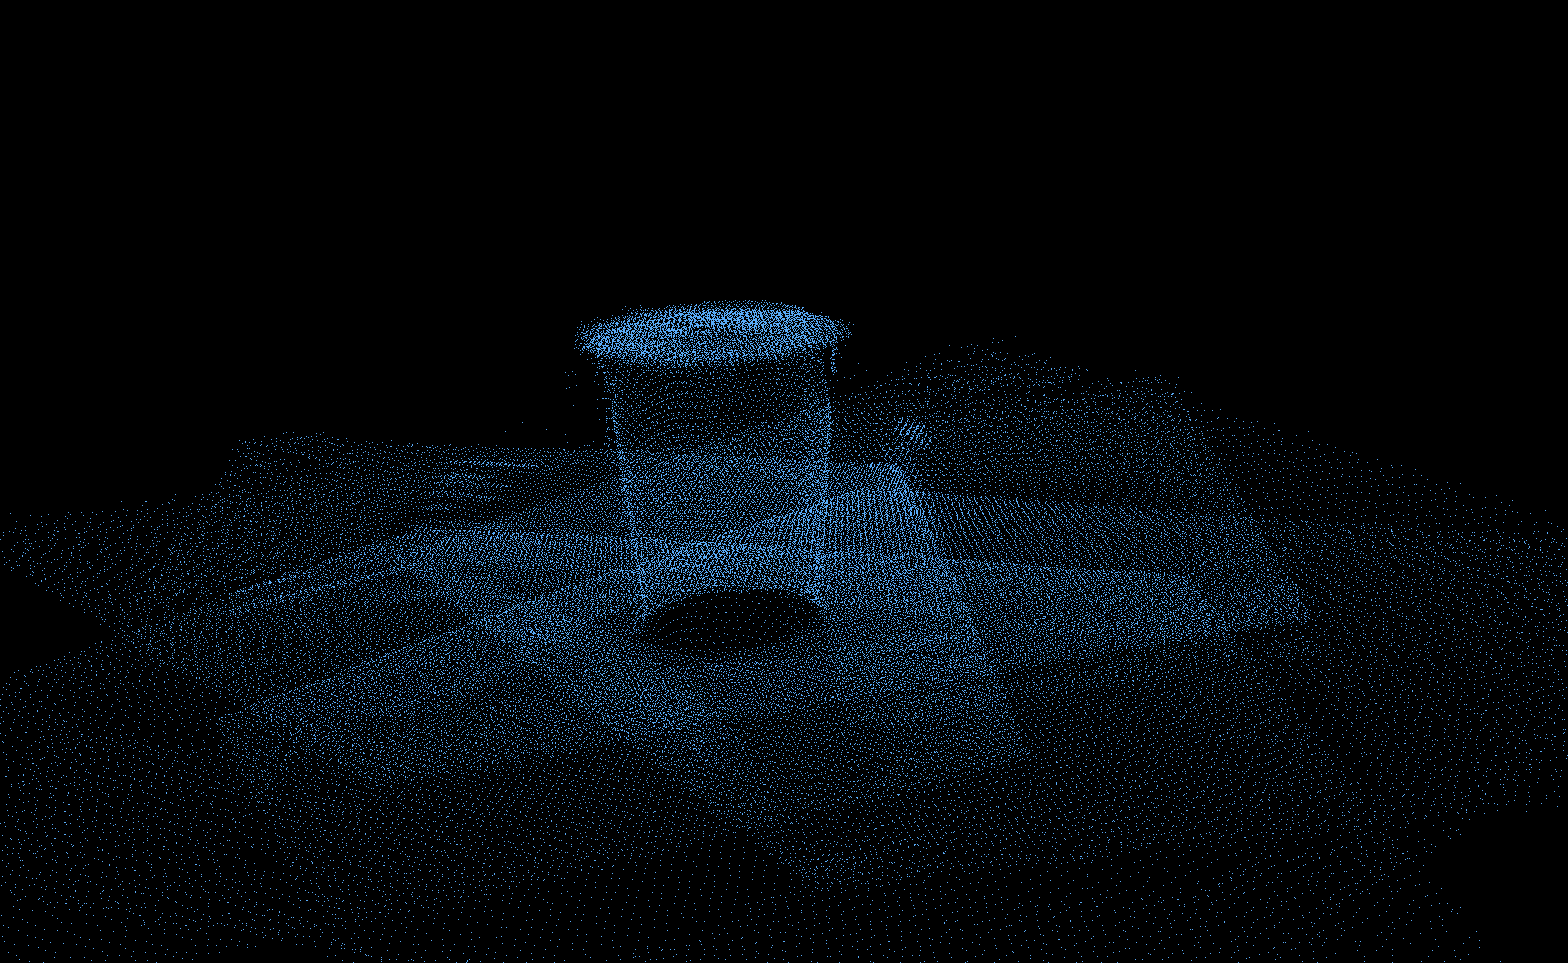
\includegraphics[width=1.0\columnwidth]{varie/point_cloud_example.png} 
    \caption{Esempio di \emph{Point Cloud}: un cestino cilindrico}
   \label{fig:point_cloud_example}
\end{figure}

\subsection{Il prototipo ad inizio stage: Samba}
In questa sezione viene presentato il prototipo nel suo stato all'inizio dello stage, per capirne le funzionalità e limiti e introdurre il lettore alle problematiche che un tale progetto sperimentale ha comportato.
Sulla base dei risultati di \emph{Samba} ho iniziato il mio lavoro sulla parte di elaborazione lato \emph{server} dei \emph{Point Cloud} acquisiti; questo stadio prototipale è stato inoltre un occasione di collaborazione con l'altro stagista e il punto di inizio per lo sviluppo del prototipo successivo.
\noindent
\emph{Samba} affronta e risolve alcuni problemi dei prototipi precedenti, come il \emph{"Drifting"} e alcuni problemi prestazionali dovuti alla mole elevata di dati acquisiti.

\subsubsection{Drift correction}
Il prototipo introduce funzionalità che tentano di arginare il problema del \emph{"drifting"}, presente in stadi prototipali precedenti. Il \emph{drifting} è un problema comune nelle applicazioni di realtà aumentata, che come \emph{Project Tango} usano la tecnica del \emph{Motion Tracking}, cioè aggiornano costantemente la propria posizione relativamente alle coordinate acquisite nella posizione precedente, mantenendo così una storia dei movimenti del \emph{device} rispetto all'ambiente circostante.\\
Ad ogni aggiornamento della posizione è normale ed inevitabile che la misurazione, per quanto precisa, introduca un piccolo errore; la catena di errori sommati porta quindi col passare del tempo ad un'importante discrepanza tra la posizione stimata del \emph{device} e la sua posizione reale, come evidenziato in figura \ref{fig:drift_correction}
\begin{figure}[!h] 
    \centering 
    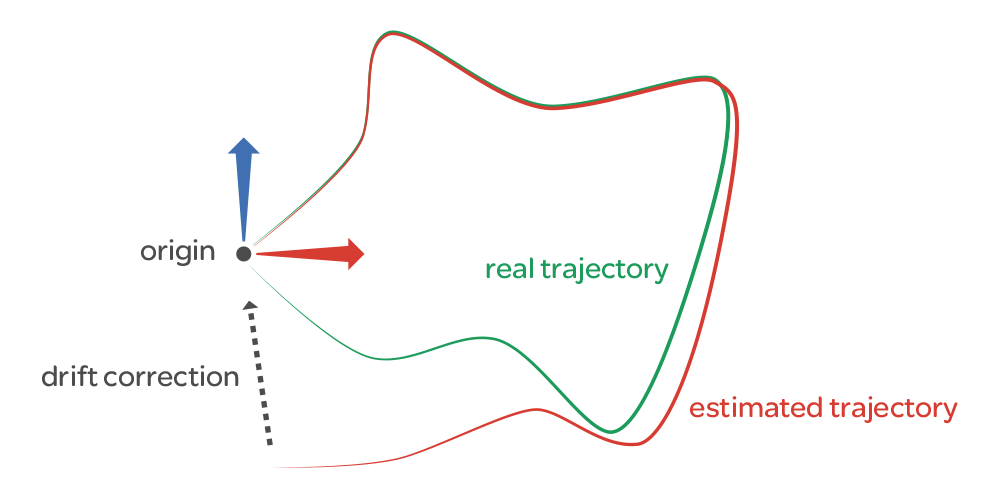
\includegraphics[width=0.9\columnwidth]{varie/Drift_Correction.png} 
    \caption{\emph{Drifting} nel \emph{Motion Tracking}}
    \label{fig:drift_correction}
\end{figure}
\newline
Per ovviare in parte a questo problema \emph{Samba} utilizza una tecnica chiamata \emph{Drift Correction} ch si appoggia sulle funzionalità di \emph{Area Learning} dei \emph{device Tango}.\\
L' \emph{Area Learning} consiste nella capacita del dispositivo di estrarre dallo spazio fisico che sta analizzando una serie di punti significativi (o \emph{key features}), facilmente riconoscibili, e di salvare tali informazioni per confrontarle con le successive acquisizioni. In questo modo il dispositivo è capace di riconoscere un'area precedentemente visitata, e può quindi applicare le necessarie correzioni alla popria stima della traiettoria, di qui il nome \emph{Drift Correction}.\\
Con l'implementazione di questa funzionalità è necessario, prima di iniziare la ricostruzione di un \emph{Point Cloud}, riprendere l'oggetto e i suoi dintorni per un po' di tempo e da diverse angolazioni, in modo da permettere al \emph{tablet Tango} di costruire una mappa, detta \emph{Area description}, dell'area circostante, e di stabilizzare la traiettoria stimata con le informazioni acquisite.\\
I risultati si vedono confrontando queste due ricostruzioni di una scatola, vista dall'alto (fig. \ref{fig:no_drift_correction} e fig. \ref{fig:with_drift_correction}), rispettivamente senza e con \emph{Drift correction}.
\begin{figure}[htp] 
    \centering
    \subfloat[Ricostruzione senza \emph{Drift correction}]{%
        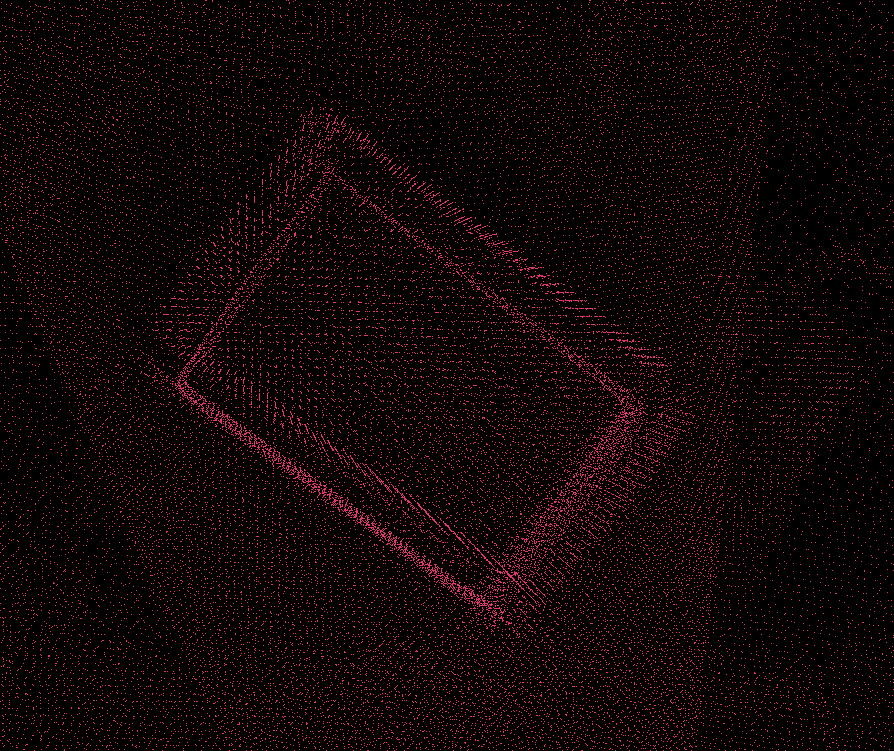
\includegraphics[width=0.47\columnwidth]{varie/no_drift_correction.png} 
    	%\caption{Ricostruzione senza \emph{Drift correction}}
    	\label{fig:no_drift_correction}
    }%
    \hfill%
    \subfloat[Ricostruzione con \emph{Drift correction}]{%
        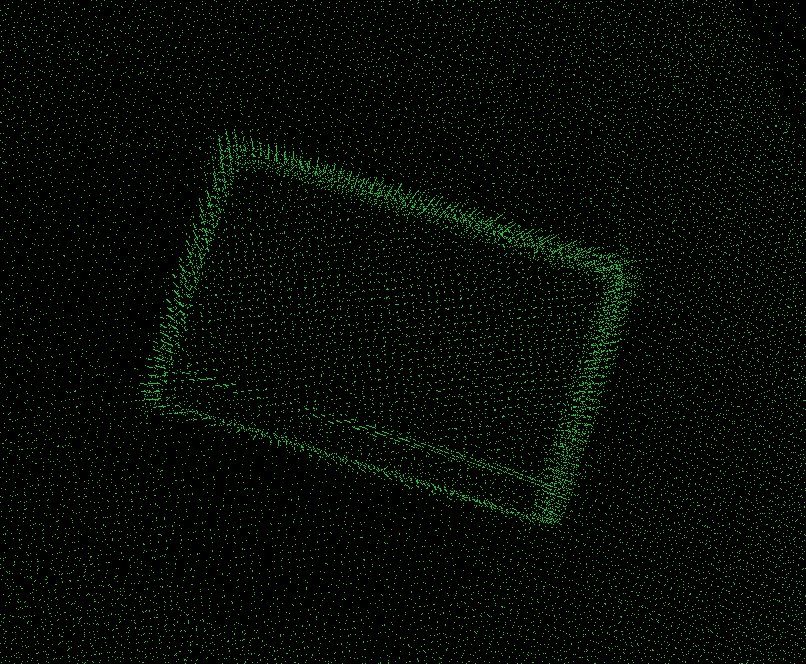
\includegraphics[width=0.47\columnwidth]{varie/with_drift_correction.png} 
    	%\caption{Ricostruzione con \emph{Drift correction}}
    	\label{fig:with_drift_correction}
    }%
    \caption{Benefici della \emph{Drift Correction}}
\end{figure}
\newline
Come si nota in figura \ref{fig:with_drift_correction} il risultato non è ancora ottimale, infatti un lato della scatola appare sdoppiato e spostato di qualche centimetro; si tratta di un problema di \emph{ghosting} di cui verrà trattato più avanti.

\subsubsection{Prestazioni}
Il prototipo precedente presentava due problemi prestazionali principali:
\begin{itemize}
\item La ricostruzione passo per passo del \emph{Point Cloud} finale era troppo lenta
\item La mole dei dati trattati al sovrapporsi di più \emph{Point Cloud} era proibitiva
\end{itemize}
\noindent
Il primo problema si presentava utilizzando i metodi forniti dalla libreria \emph{Tango} per trasformare le coordinate relative dei punti in coordinate assolute per permetterne la giusta sovrapposizione. Tale metodo, seppur di facile utilizzo, diventava troppo dispendioso all'aumentare delle dimensioni del \emph{Point Cloud}, che raggiunge facilmente gli 80.000 punti.\\
Per risolvere il problema viene quindi creata, per ogni \emph{Point Cloud}, una \emph{matrice di rototraslazione} che rappresenta lo spostamento e la rotazione del dispositivo rispetto al sistema di riferimento, e viene moltiplicato il vettore delle coordinate di ogni singolo punto per la matrice generata. \\
In questo modo si sono ridotti i tempi di elaborazione dell'80\%;
\newline

\noindent
Il secondo problema era causato dal sovrapporsi di molti punti quasi identici, ad esempio i punti rappresentanti il pavimento. Partendo dall'osservazione che una certa quantità di punti molto vicini può essere trasformata in un unico punto, valore medio di tutti gli altri, senza una significativa perdita d'informazione, \emph{Samba} risolve il problema attraverso una tecnica di \emph{voxeling}.\\
Lo spazio viene suddiviso in tanti piccoli parallelepipedi (tipicamente cubi) di uguali dimensioni; tutti i punti che ricadono all'interno di un singolo parallelepipedo, o \emph{voxel}, vengono considerati come un unico punto. Così facendo si riducono sensibilmente le dimensioni del \emph{Point Cloud} senza alterarne negativamente la precisione.
Di seguito la differenza visivamente evidente tra lo stesso Point Cloud filtrato prima con voxel cubici di lato 1cm (fig. \ref{fig:low_voxeling}) e poi di lato 3cm (fig. \ref{fig:high_voxeling}), con una differenza di circa 60.000 punti rimossi in più nella seconda elaborazione.
\begin{figure}[htp] 
    \centering
    \subfloat[Voxeling leggero]{%
        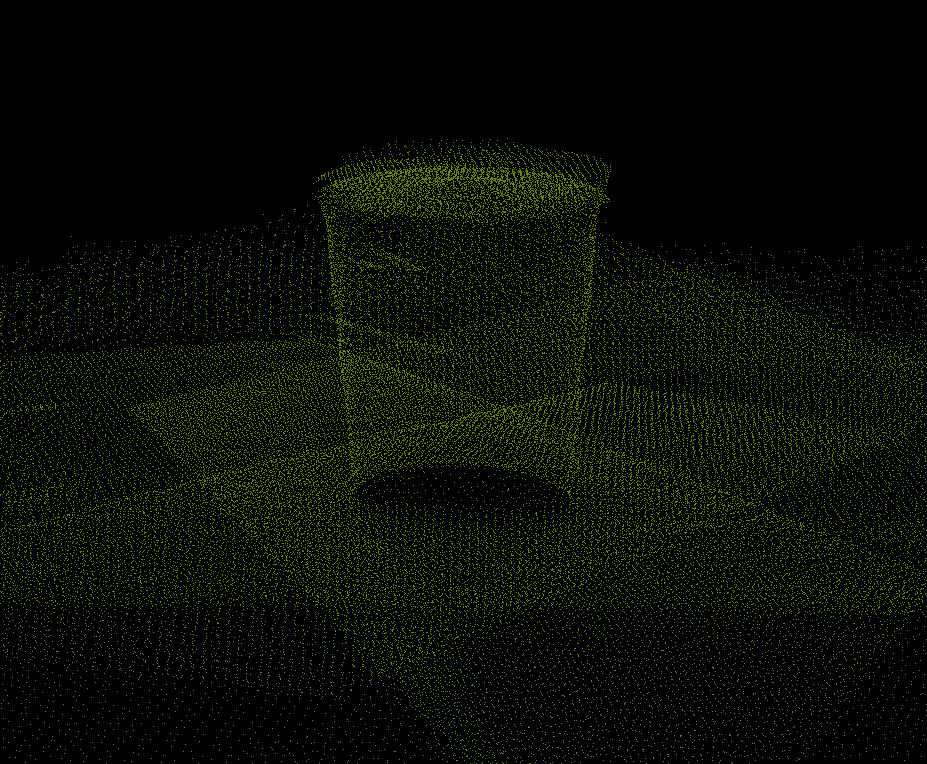
\includegraphics[width=0.47\columnwidth]{varie/low_voxeling.png} 
    	\label{fig:low_voxeling}
    }%
    \hfill%
    \subfloat[Voxeling elevato]{%
        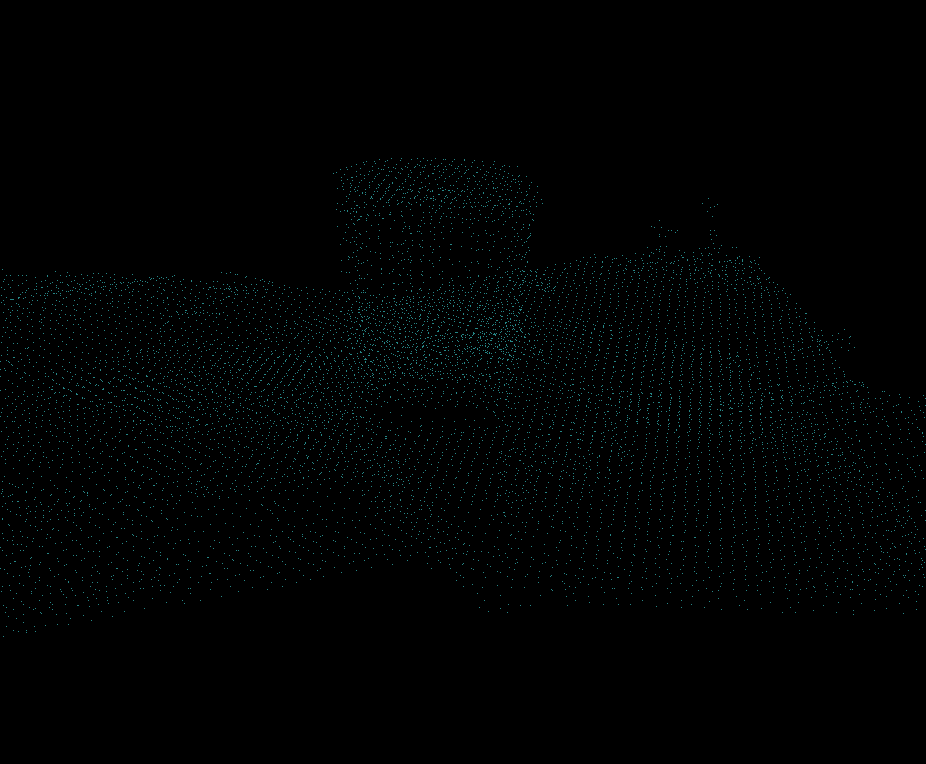
\includegraphics[width=0.47\columnwidth]{varie/high_voxeling.png} 
    	\label{fig:high_voxeling}
    }%
    \caption{Effetti del \emph{voxeling}}
\end{figure}
\newline

%\subsection{L'applicativo attuale: VIC-Tango}
%L'ultimo prototipo si avvicina già ad uno stato più stabile e funzionale e si pone come base su cui sviluppare l'applicazione in futuro. VIC-Tango è una versione rifinita e migliorata di \emph{Samba}, della quale sono stati risolti svariati bug, immancabili allo stadio prototipale. Introduce inoltre alcune nuove funzionalità che migliorano la User experience e lasciano la porta aperta a sviluppi futuri.
%
%\subsubsection{Firebase}
%\emph{Firebase} è un \emph{framework} associato all'omonimo \emph{web service} offerto da \emph{Google} per lo scambio di messaggi tra applicazioni \emph{Android} e un \emph{server}. In particolare è stato utlizzato il servizio \emph{Firebase} di cloud messaging per la gestione e invio affidabile di messaggi a più dispositivi differenti.\\ Il suo utilizzo in VIC-Tango ha permesso di implementare un servizio di notifica da parte del server, che può così inviare messaggi asincroni al device Tango, il quale li riceverà come notifica di sistema Android, informandolo ad esempio che il Point Cloud inviato è stato elaborato e una nuova mesh è stata generata. L'utente può così continuare l'ispezione e acquisire nuovi Point Cloud e, alla ricezione della notifica, caricare e visualizzare automaticamente le mesh quando disponibili.
%
%\subsubsection{Camera preview}
%Fin dal prototipo precedente era stata introdotta una piccola preview di quanto ripreso dalla fotocamera RGB-IR. Tuttavia la funzionalità era stata implementata utilizzando una soluzione general-purpose applicabile a più dispositivi Android, che causava però problemi prestazionali e crash occasionali dell'applicativo. \\
%La preview è stata quindi reimplementata utilizzando le funzionalità esposte dalle Tango API, soluzione inizialmente scartata perchè quest'ultime erano mal documentate, ottenendo un miglioramento delle prestazioni e la correzione dei bug rilevati.
%
%\subsubsection{Visualizzatore di mesh}
%Nel prototipo è stata introdotta la possibilità di caricare e visualizzare le \emph{mesh} risultato dell'elaborazione lato server di un \emph{Point Cloud}.
%Una \emph{mesh} poligonale è una collezione di vertici, spigoli e facce che definiscono la forma di un oggetto poliedrico; in \emph{Samba} è ottenuta a partire dalla nuvola di punti elaborata.
%Tale \emph{mesh} viene salvata dal \emph{server} in formato \emph{OBJ}, comunemente usato nelle applicazioni 3D. Dall'applicazione viene quindi richiesto di caricare e salvare nella memoria locale del tablet le mesh disponibili sul server, per poi poter essere visualizzate ed esaminate.
%
%\subsubsection{JNI e Point Cloud Registration}
%La Java Native Interface o JNI è un framework del linguaggio Java che consente al codice Java di richiamare codice cosiddetto "nativo", ovvero specifico di un determinato sistema operativo scritto in altri linguaggi di programmazione, in particolare C/C++.\\
%L'integrazione della JNI con lo sviluppo Android, in particolare il suo utilizzo nell'IDE Android Studio, è un compito tutt'altro che semplice, dato il supporto ancora scarso all'integrazione del framework con l'IDE e il build-tool Gradle.\\
%Dopo svariati tentativi iniziati già i primi giorni di stage, quindi già dai prototipi precedenti, è stato infine possibile usufruire della JNI utilizzando versioni sperimentali di Android Studio e Gradle. \\
%Attraverso la JNI si è provato ad importare la libreria PCL, così da poterne utilizzare le potenti funzionalità direttamente dal tablet. Purtroppo l'integrazione con il build-tool Gradle richiede un makefile apposito, compito improponibile per una libreria notevolmente complessa come PCL, le cui potenzialità sono quindi rimaste nel lato server.\\
%Si è riuscito invece ad importare, date le ridotte dimensioni, una libreria per la \emph{Registration} di Point Cloud. Col termine \emph{Registration} si indica il processo che trasforma in coordinate assolute e allinea due set di Point Cloud in un unico set che minimizza le distanze tra punti corrispondenti (ad es. fig. \ref{fig:reg_example}).
%\begin{figure}[!h] 
%    \centering 
%    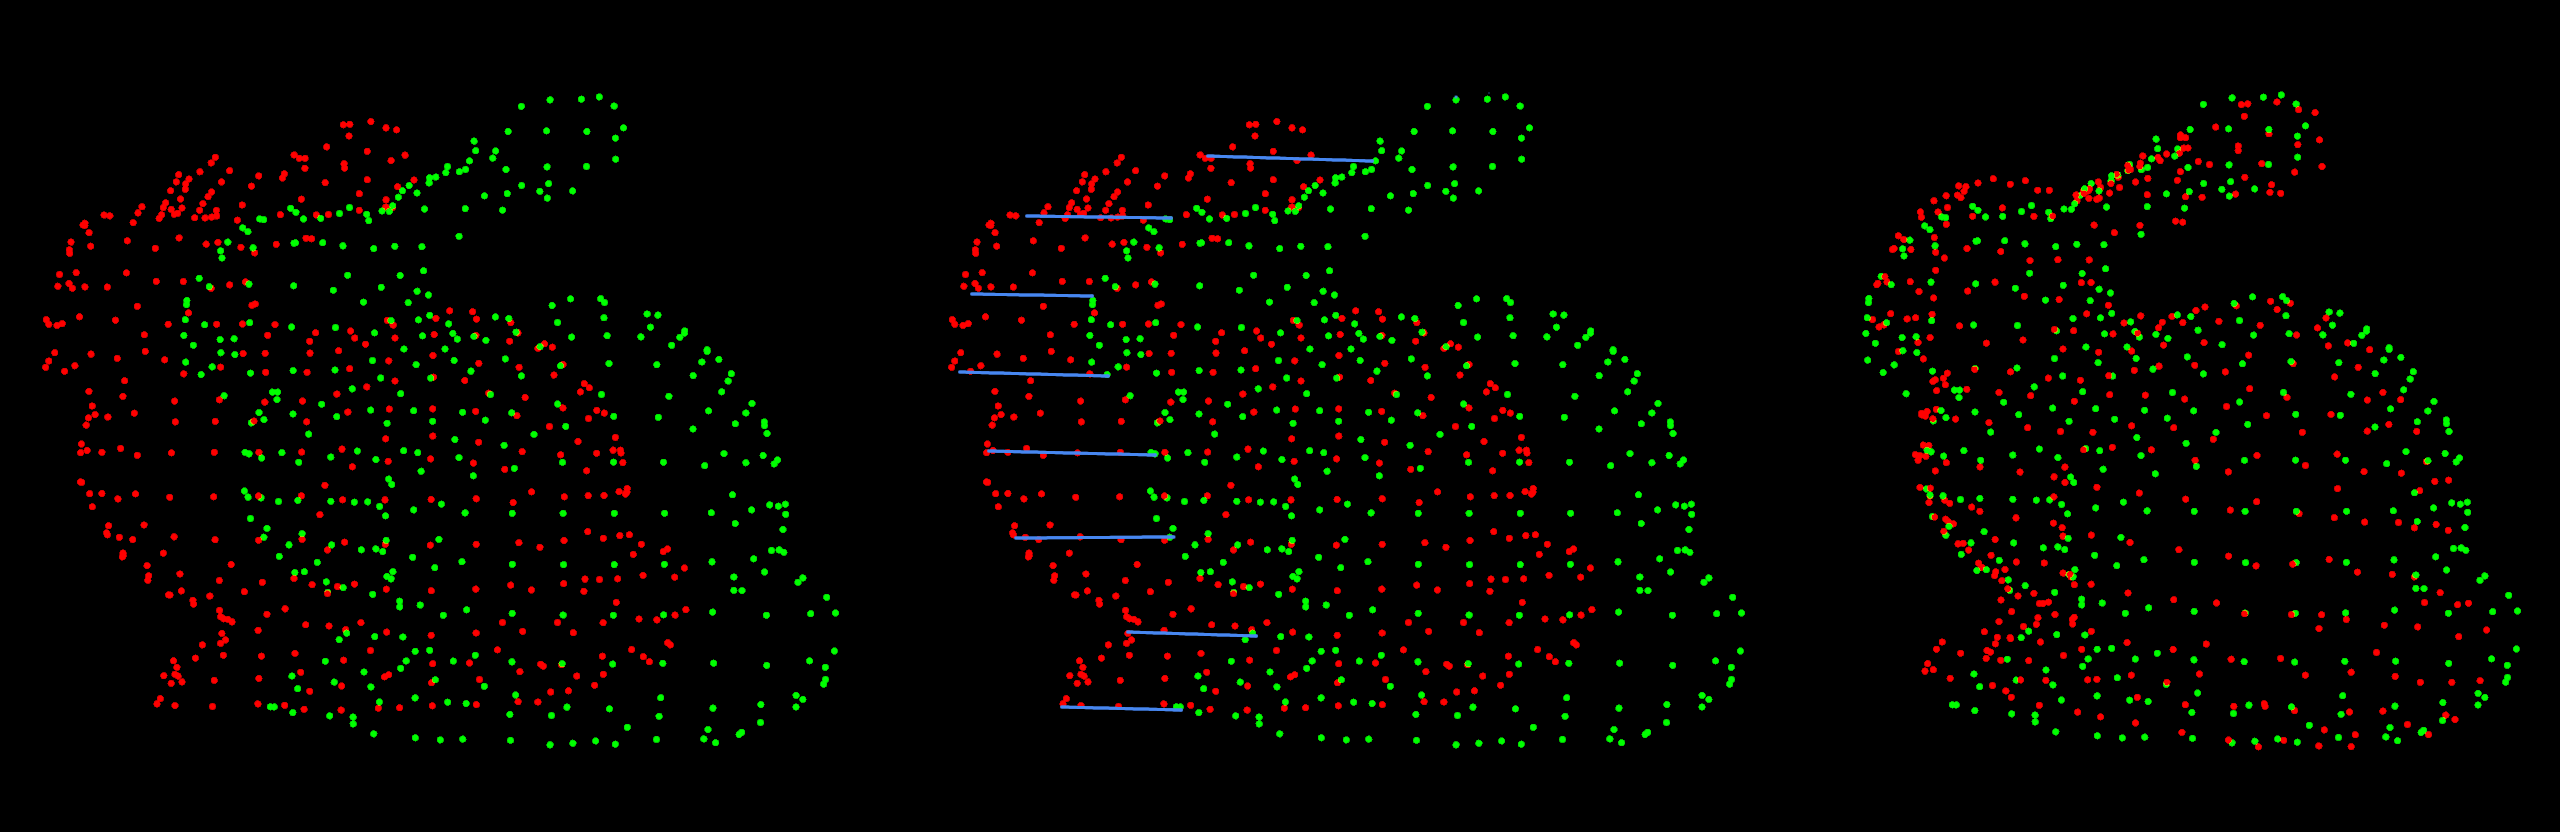
\includegraphics[width=1.0\columnwidth]{varie/registration_example.png} 
%    \caption{\emph{Point Cloud Registration} tramite l'algoritmo \emph{ICP}}
%    \label{fig:reg_example}
%\end{figure}
%\newline
%La libreria in questione, GOICP, implementa una versione ottimizzata dell'algoritmo ICP (Iterative Closest Point), spesso utilizzato in applicazioni nelle quali sia necessario ricostruire una superficie tridimensionale a partire da più scansioni, che punta a minimizzare la distanza tra i punti delle due Point Cloud.\\
%L'algoritmo ICP tenta di minimizzare l'errore quadratico medio (in inglese Mean Squared Error, MSE) cioè la discrepanza quadratica media fra i valori dei punti della coppia di Point Cloud, definita come:
%$$
%	MSE = \displaystyle\frac{\sum_{i=1}^{n} (x_i - x'_i)^2}{ n }
%$$
%Si è testato GOICP sulle coppie di Point Cloud acquisite con VIC-Tango, per ovviare al problemi già presentati del \emph{drifting} (fig. \ref{fig:no_drift_correction}) e del \emph{ghosting} (fig. \ref{fig:with_drift_correction}); si sono ottenuti però risultati insoddisfacenti. Sono sorti infatti i seguenti problemi:
%\begin{itemize}
%\item Il processo è eccessivamente dispendioso da effettuare su tablet, con tempi di elaborazione tra i 10 e i 60 secondi.
%\item L'algoritmo ICP, basandosi sul MSE come valore di bontà, converge spesso lentamente e  a soluzioni errate, per colpa della grande quantità di punti planari sul pavimento, che rendono l'errore quadratico medio un valore non attendibile su cui basare il successo di una \emph{Registration} 
%\end{itemize}
%Come si vede in figura \ref{fig:goicp} l'algoritmo, pur ottenendo un basso valore di MSE, non effettua la \emph{Registration} desiderata, dato che vengono allineati perlopiù i punti planari.
%\begin{figure}[htp] 
%    \centering
%    \subfloat[Prima scansione]{%
%        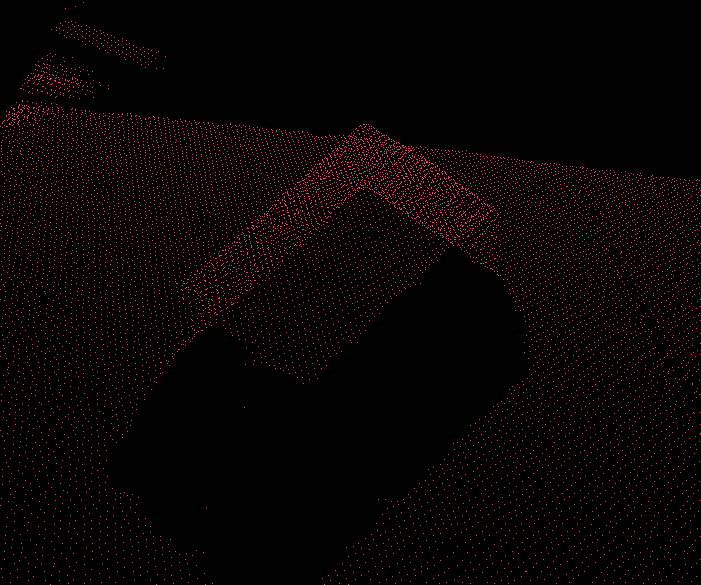
\includegraphics[width=0.5\columnwidth]{varie/to_align_left.png} 
%    	\label{fig:goicp_left}
%    }%
%    \hfill%
%    \subfloat[Seconda scansione]{%
%        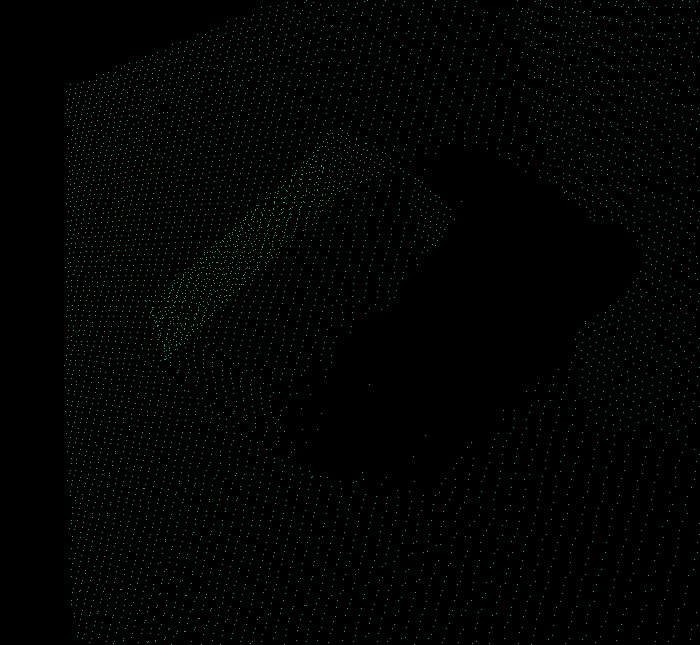
\includegraphics[height=0.42\columnwidth]{varie/to_align_right.png} 
%    	\label{fig:goicp_right}
%    }%
%    \hfill%
%    \subfloat[Risultato di GOIPC]{%
%        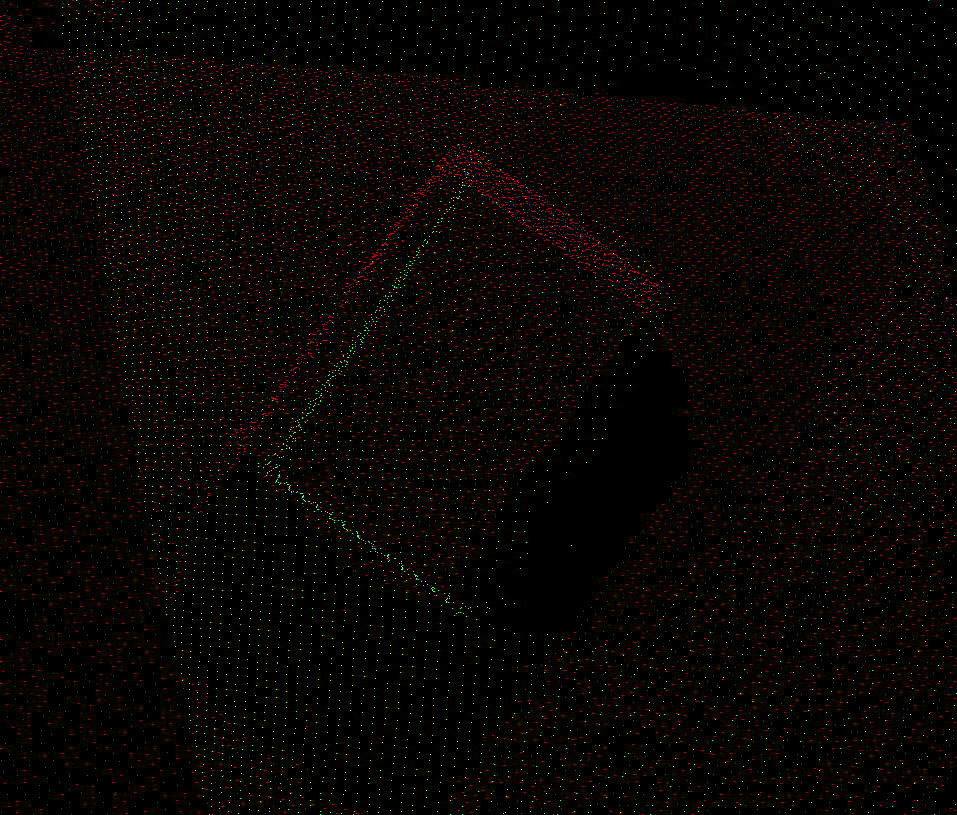
\includegraphics[width=0.6\columnwidth]{varie/goicp.png} 
%    	\label{fig:goicp}
%    }%
%    \caption{Errore nella \emph{Registration} con \emph{GOICP}}
%\end{figure}
%\newline
%
%\noindent
%Per questi motivi la \emph{registration} tramite GOICP è rimasta in uno stadio prototipale, che necessita di almeno una delle seguenti correzioni:
%\begin{itemize}
%\item Trovare una misura più adatta del MSE per valutare la convergenza dell'algoritmo ICP
%\item Alternativamente, eliminare dal Point Cloud i punti planari appartenenti al pavimento così da poter utilizzare l'errore quadratico medio come affidabile valore di convergenza
%\item Ottimizzare GOICP o implementare un algoritmo ICP ad hoc per ridurre drasticamente i tempi di elaborazione
%\end{itemize}
%\noindent
%Tali correzioni trattano problemi non triviali, che l'esiguo tempo di tirocinio rimasto non mi ha permesso di affrontare adeguatamente. La Point Cloud Registration rimane quindi una funzionalità necessaria ad assicurare un'affidabile e corretta ricostruzione degli oggetti scansionati, aperta a sviluppi futuri.



%**************************************************************
%\section{Il Prodotto - lato server}
%Il lato server dell'applicazione si occupa di ricevere dai \emph{Tango device} i Point Cloud acquisiti, elaborarli utilizzando la libreria PCL per estrarre i punti rappresentanti il solo oggetto scansionato, produrre una mesh dell'oggetto così ottenuto e calcolarne il volume. Invia poi quando necessario i risultati elaborati ai dispositivi che li richiedono.\\
%Quando un Point Cloud viene ricevuto dal server tramite una richiesta HTTP POST, inserito in un oggetto JSON, viene salvato in un file PCD. Il formato PCD (Point Cloud Data) usato nella libreria PCL è molto semplice: è formato da un header contenente alcune informazioni utili come il numero totale di punti e il tipo e numero di valori associati ad ogni punto; segue poi l'effettivo Point Cloud codificato riga per riga, dove ogni riga contiene una successione di valori che rappresenta un punto.\\
%Il file salvato viene poi elaborato sfruttando la libreria PCL.
%
%\subsection{Point Cloud Library}
%\emph{PCL} o \emph{Point Cloud Library} è una libreria \emph{Open Source}, scritta in C++, di algoritmi per l'elaborazione di \emph{Point Cloud} tridimensionali. Contiene algoritmi per il filtraggio, la segmentazione, la \emph{registration} e il \emph{meshing} di Point Cloud, per citarne alcuni. \\
%La libreria è ampiamente utilizzata da qualsiasi applicativo debba trattare nuvole di punti, ed oltre ad essere utile ed efficiente è anche ben documentata, con molti esempi d'utilizzo reperibili online.\\
%Le notevoli potenzialità della libreria sono state utilizzate intensivamente nell'applicativo con lo scopo di isolare i punti appartenenti all'oggetto scansionato dal resto del Point Cloud, ed effettuarne quindi il meshing.
%
%\subsection{Elaborazione di un Point Cloud}
%
%La nuvola di punti salvata in un file PCD viene elaborata da un applicativo scritto in C++ che sfrutta le numerose funzionalità della PCL.
%L'elaborazione di un Point Cloud è composta di più passi sequenziali:
%\begin{enumerate}
%\item Viene caricato il nuovo Point Cloud da file PCD salvato localmente
%\item Vengono rimossi i punti isolati della nuvola attraverso la libreria Sparse Filtering
%\item Vengono rimossi i punti troppo esterni della nuvola attraverso la libreria Radius Filtering 
%\item Vengono rimossi i punti che corrispondono al piano del pavimento attraverso la libreria Ground Filtering
%\item Viene effettuato il \emph{downsample} del \emph{dataset} attraverso la libreria Voxel Filtering
%\item Viene estratto il cluster maggiore dai punti rimanenti attraverso la libreria Cluster Extraction
%\item Viene effettuato il meshing del cluster estratto, e la mesh viene salvata in due file OBJ (per la visualizzazione lato client) e VTK (per il calcolo del volume)
%\item Viene calcolato e salvato il volume della mesh prodotta
%\end{enumerate}
%Per ogni passo di filtraggio la nuvola di punti viene salvata su un distinto file PCD, per poter analizzare visivamente la bontà dell'elaborazione.
%Di seguito vengono descritti in dettaglio filtri applicati e il processo di meshing.
%
%\subsubsection{Sparse filtering}
%Questo primo passo di filtraggio si occupa di rimuovere dal Point Cloud i punti isolati. Per ogni punto viene effettuata una analisi statistica della distanza media dai suoi vicini. I punti la cui distanza dai vicini supera un certo valore sono quindi isolati e possono essere eliminati dalla nuvola.
%Un esempio di tale tecnica, sul quale si basa l'implementazione di questo filtro, è lo "Statistical Outlier Removal\footcite{http://pointclouds.org/documentation/tutorials/statistical_outlier.php/statistical-outlier-removal}" di PCL.\\
%In figura \ref{fig:sparse} vediamo i risultati di tale filtro, con una rimozione di circa 10.000 punti.
%\begin{figure}[!h] 
%    \centering 
%    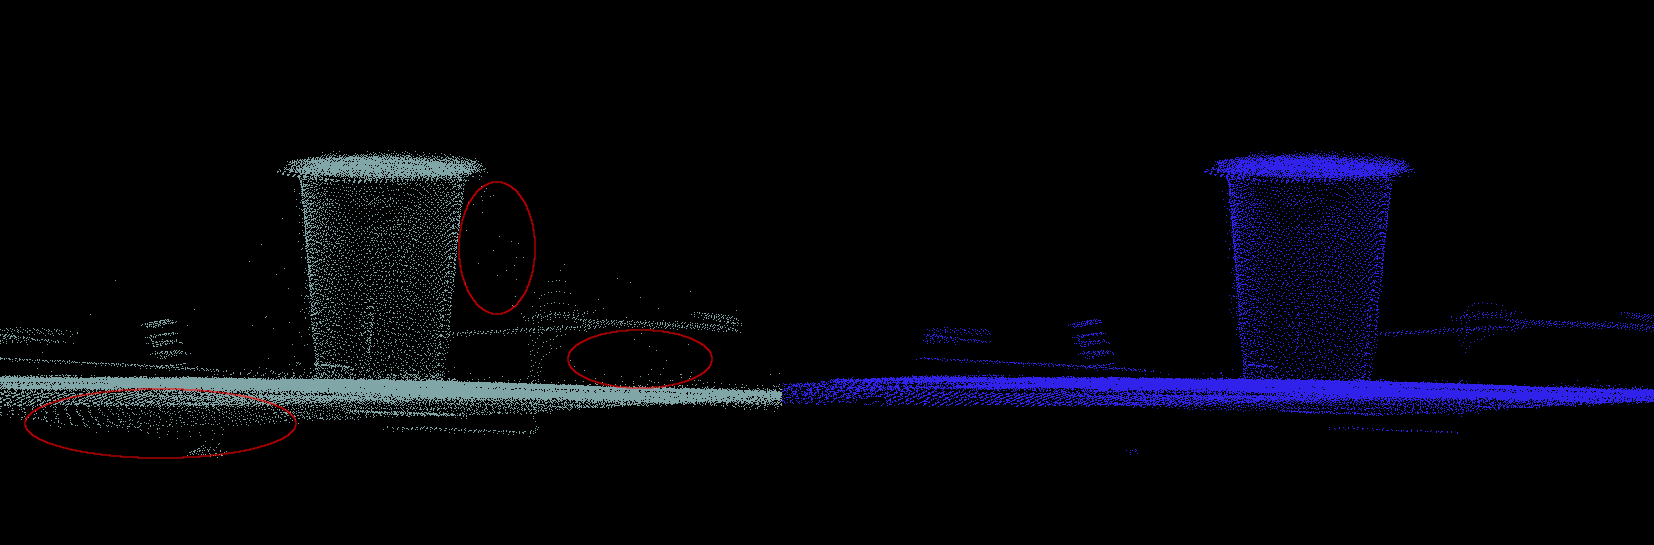
\includegraphics[width=1.0\columnwidth]{varie/sparse.png} 
%    \caption{\emph{Sparse filtering}}
%    \label{fig:sparse}
%\end{figure}
%\subsubsection{Radius filtering}
%Questo passo di filtraggio si occupa di eliminare i punti troppo distanti dal centro, che solitamente appartengono alle pareti circostanti o comunque ad oggetti diversi da quello scansionato, che sarà sempre verso il centro della nuvola.\\
%Partendo da questo presupposto, il filtro calcola il punto centrale del Point Cloud, media del valore di tutti i punti, e procede con l'eliminare i punti che superano una certa distanza (\emph{radius}), attraverso l'algoritmo PCL "PassThrough Filter\footcite{http://pointclouds.org/documentation/tutorials/passthrough.php/passthrough}", fino a che non è stata eliminata una definita percentuale del point set iniziale.\\
%In figura \ref{fig:radius} vediamo i risultati di tale filtro, con una rimozione di circa 24.000 punti.
%\begin{figure}[!h] 
%    \centering 
%    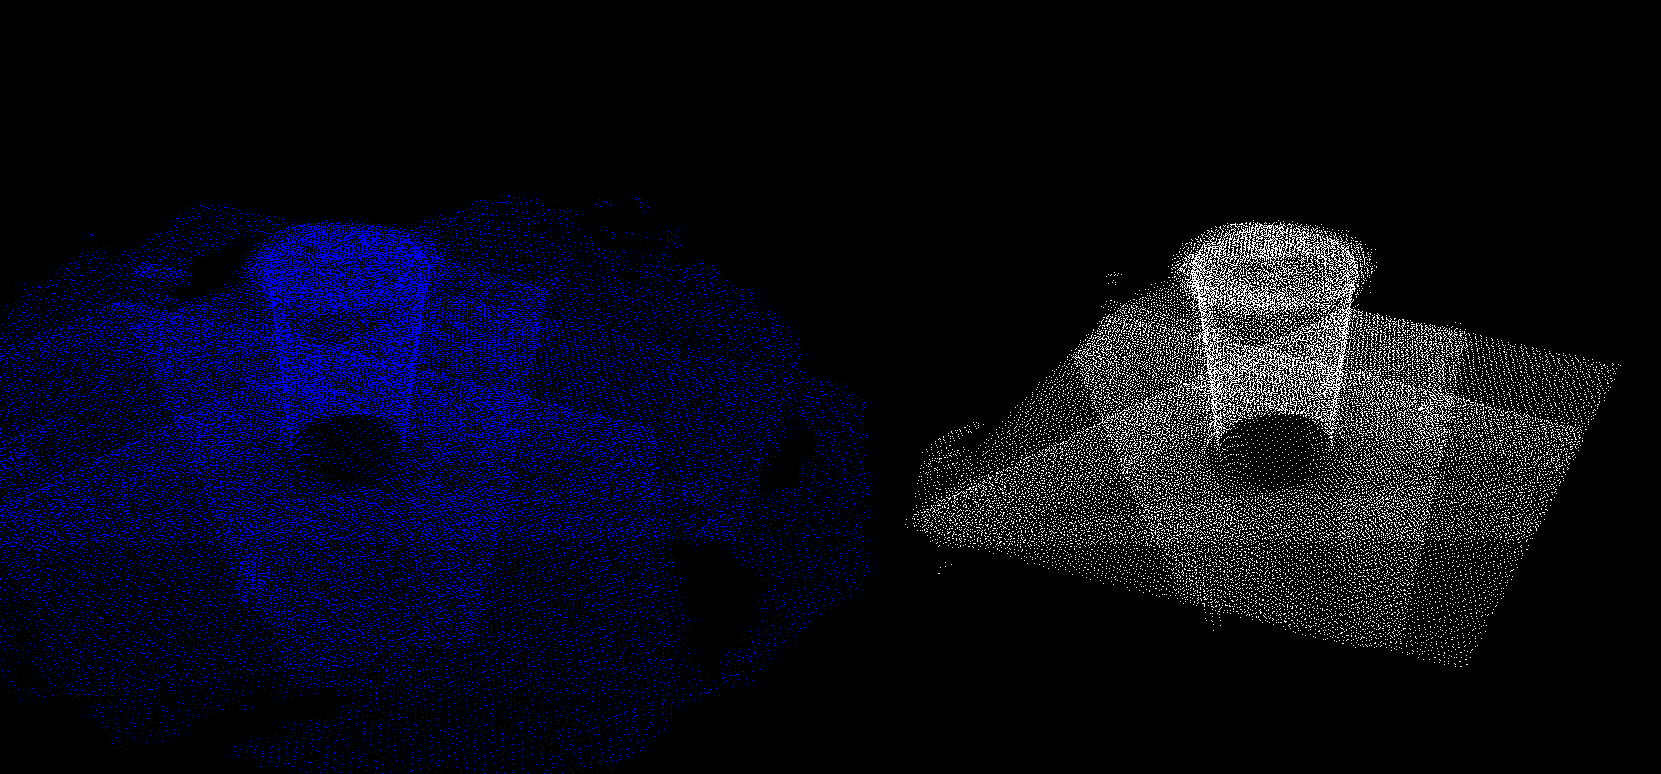
\includegraphics[width=1.0\columnwidth]{varie/radius.png} 
%    \caption{\emph{Radius filtering}}
%    \label{fig:radius}
%\end{figure}
%\subsubsection{Ground filtering}
%Questo passo di filtraggio si occupa di eliminare i punti planari appartenenti al pavimento, problema che si è rilevato essere uno dei più difficili da trattare. 
%In primo luogo non sempre c'è un unico componente planare che rappresenta il pavimento, ma solitamente ve n'è più d'uno, a causa delle imprecisioni nell'acquisizione dei Point Cloud lato client. Per l'implementazione del filtro si è fatto uso degli algoritmi di \emph{segmentation} di PCL (ad es. "Planar segmentation\footcite{http://pointclouds.org/documentation/tutorials/planar_segmentation.php}"), che consentono di estrarre i punti della nuvola che giacciono sullo stesso piano. Senza ulteriori aggiustamenti però l'algoritmo elimina anche piani utili, come il lato superiore di una scatola o di un tavolo.
%Si è reso quindi necessario applicare i seguenti passi:
%\begin{enumerate}
%\item Calcolare l'altezza del Point Cloud e dividere la parte superiore da quella inferiore, che deve contenere il pavimento
%\item Applicare l'algoritmo di \emph{planar segmentation} alla sotto-nuvola estratta fino a che non è stato eliminato un numero adeguato di punti
%\item Ricongiungere la parte inferiore filtrata alla parte superiore del Point Cloud
%\end{enumerate}
%Il filtro così impostato ottiene ottimi risultati nella maggior parte dei casi. Tuttavia se il Point Cloud originale presenta troppo  \emph{drifting}, e i piani del pavimento sono molto distanti tra loro, diventa impossibile eliminarli senza togliere anche punti importanti dell'oggetto scansionato.\\
%In figura \ref{fig:ground} vediamo i risultati di tale filtro, applicato ad un Point Cloud già sottoposto ai filtri precedenti, con una rimozione di circa 50.000 punti.
%\begin{figure}[!h] 
%    \centering 
%    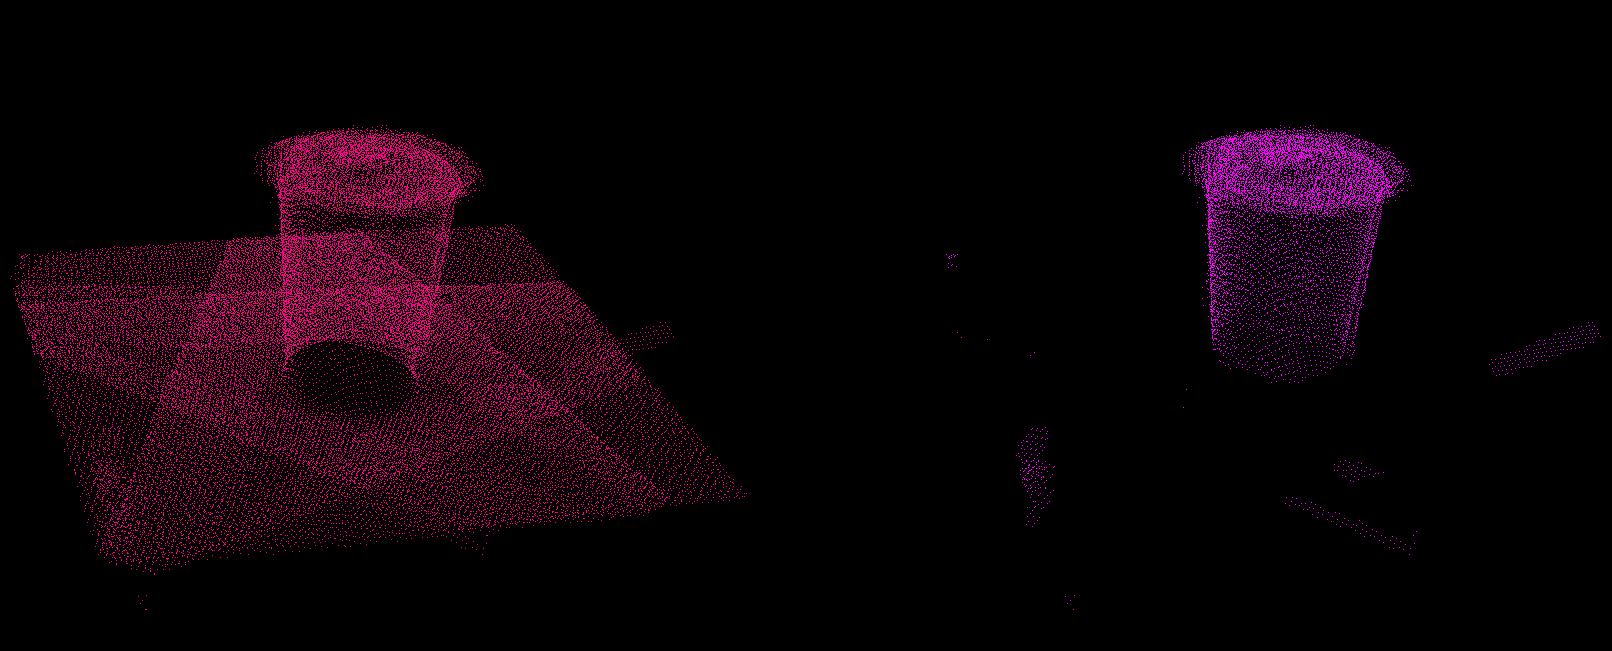
\includegraphics[width=1.0\columnwidth]{varie/ground.png} 
%    \caption{\emph{Ground filtering}}
%    \label{fig:ground}
%\end{figure}
%
%\subsubsection{Voxel filtering}
%Questo passo di filtraggio si occupa di eliminare i punti doppi e ridurre le dimensioni del Point Cloud per il futuro meshing. Il filtro utilizza la stessa tecnica già implementata nel lato client, cioè suddividere lo spazio in tanti \emph{voxel} cubici e  calcolare il punto medio di ogni voxel come approssimazione dei punti che ricadono al suo interno. L'implemetazione prende spunto dall'esempio di PCL "VoxelGrid Filter\footcite{http://pointclouds.org/documentation/tutorials/voxel_grid.php}".
%Per i risultati del \emph{voxel filtering} si rimanda alle figure \ref{fig:low_voxeling} e \ref{fig:high_voxeling}.
%\subsubsection{Cluster extraction}
%L'ultimo passaggio prima del meshing è il \emph{Cluster extraction}, cioè il completo isolamento della nuvola di punti rappresentante oggetto in ispezione.
%L'algoritmo PCL "\emph{Euclidean Cluster Extraction\footcite{http://www.pointclouds.org/documentation/tutorials/cluster_extraction.php}}" su cui si base quest'ultimo step di filtraggio suddivide lo spazio del Point Cloud in più parti ed analizzandone statisticamente la densità per ogni parte, riesce a determinare quali sono  gli aggregati di punti nella nuvola, distinguibili gli uni dagli altri.
%L'algoritmo suddivide quindi la nuvola in più cluster, e ne estrae quello di maggiori dimensioni. Questo filtraggio finale indispensabile al passo successivo di meshing, perchè elimina dal Point Cloud tutti gli elementi estranei all'oggetto.\\
%In figura \ref{fig:cluster} vediamo i risultati di tale filtro, applicato ad un Point Cloud già sottoposto ai filtri precedenti, con una rimozione di circa 4.000 punti. Sono evidenziati in figura alcuni piccoli gruppi di punti che è necessario eliminare, che rappresentano degli artefatti inesistenti nel mondo reale, ma che sono immancabilmente presenti nelle scansioni di un oggetto. L'origine di tali anomalie non è ancora chiara, probabilmente sono causate da riflessi del pavimento.
%\begin{figure}[!h] 
%    \centering 
%    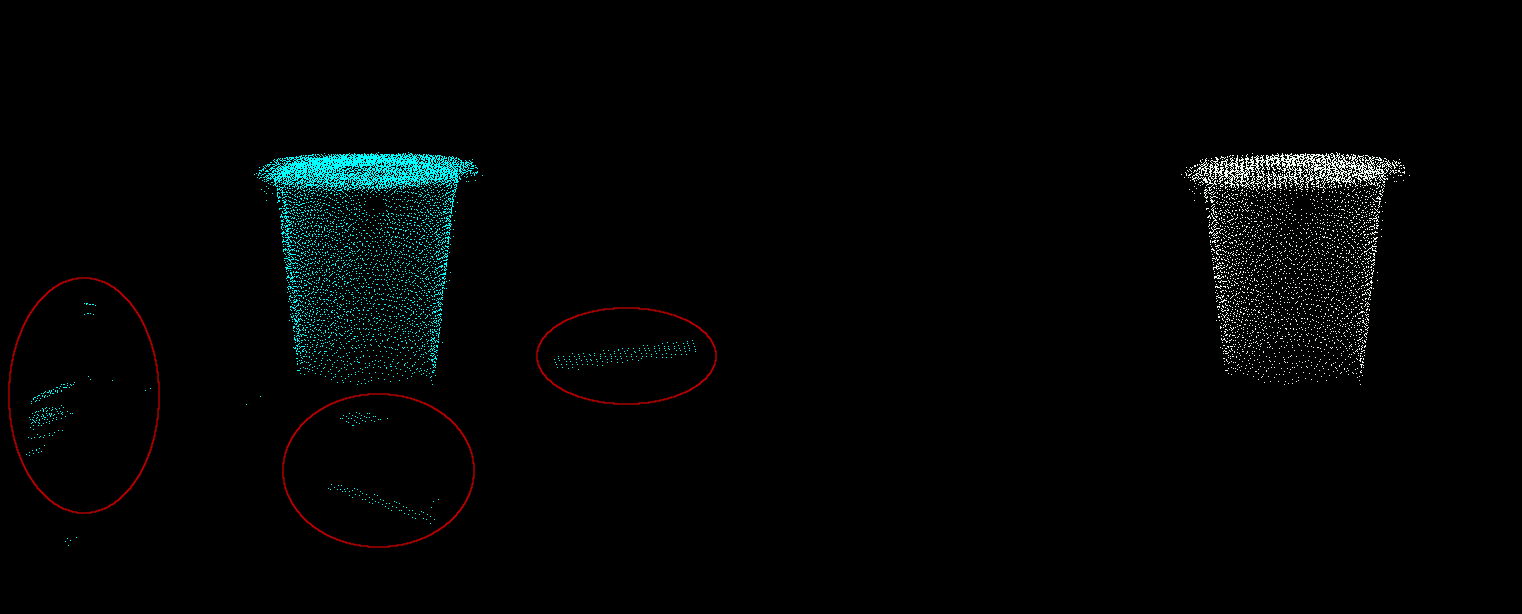
\includegraphics[width=1.0\columnwidth]{varie/cluster.png} 
%    \caption{\emph{Cluster extraction}}
%    \label{fig:cluster}
%\end{figure}
%
%\subsubsection{Meshing}
%Una volta ottenuti i punti della nuvola rappresentanti il solo oggetto scansionato, si può procedere col generarne una mesh tridimensionale.
%Il processo sfrutta un algoritmo greedy di PCL, la "\emph{Greedy Projection Triangulation\footcite{http://www.pointclouds.org/documentation/tutorials/greedy_projection.php}}", che, connettendo ogni punto ai propri vicini, genera un mesh composta da migliaia di triangoli che approssima la superficie reale dell'oggetto.
%In figura \ref{fig:mesh} vediamo i risultati del processo di meshing applicato ad un Point Cloud già sottoposto ai filtri precedenti.
%\begin{figure}[!h] 
%    \centering 
%    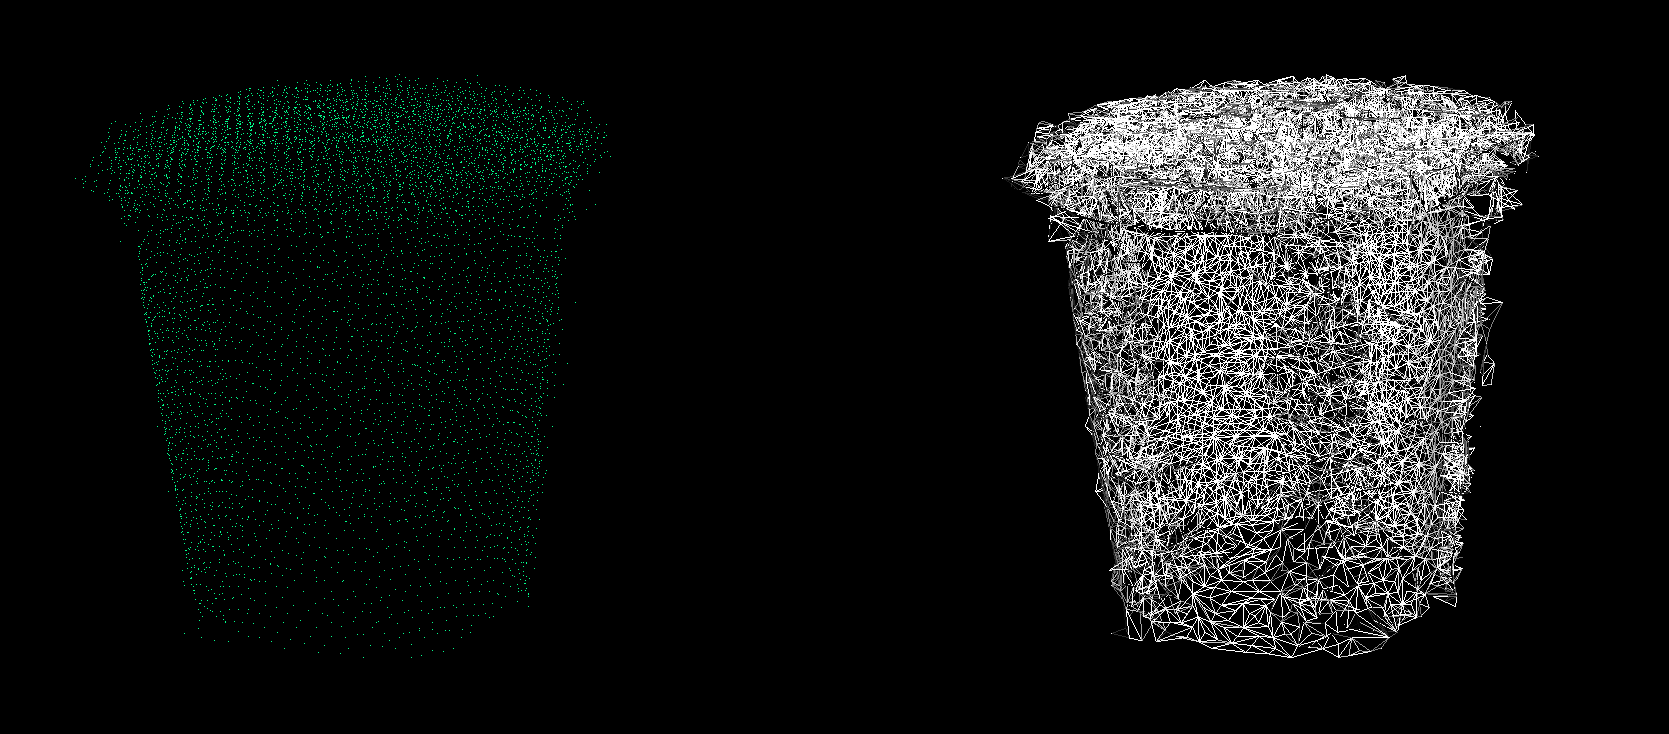
\includegraphics[width=1.0\columnwidth]{varie/mesh.png} 
%    \caption{\emph{Meshing} di un \emph{Point Cloud}}
%    \label{fig:mesh}
%\end{figure}
%\newline
%La mesh così ottenuta non è una superficie chiusa, spesso infatti le scansioni non riescono a catturare tutti i punti di un oggetto, e manca completamente il piano di base dell'oggetto scansionato, che non è possibile rilevare. Ciò non influisce particolarmente sul successivo calcolo del volume.
%
%\subsection{Calcolo del volume}
%Una volta generata la mesh è possibile calcolarne il volume sfruttando il risultato pubblicato da Cha Zhang e Tsuhan Chen nel loro paper\footcite{http://research.microsoft.com/en-us/um/people/chazhang/publications/icip01_ChaZhang.pdf}. Viene calcolato, per ogni triangolo che compone la \emph{mesh}, il volume con segno del tetraedro che ha il triangolo stesso come base e il quarto vertice in un punto fissato, scelto internamente alla \emph{mesh}, per evitare eventuali problemi di instabilità numerica. Il segno del volume è dato dalla direzione della normale al piano del triangolo. Questi volumi, sommati tra loro, restituiscono il volume convesso della \emph{mesh}.\\
%Il calcolo del volume, nella sua semplicità e velocità d'elaborazione, pone però delle condizioni sulla qualità della mesh:
%\begin{itemize}
%\item La superficie non necessita di essere chiusa, ma il calcolo ne beneficierebbe
%\item Il punto scelto come quarto vertice del tetraedro deve appartenere alla mesh
%\item La mesh non deve contenere triangoli che si sovrappongono o si intersecano
%\end{itemize}
%La bontà del calcolo dipende quindi molto dalla qualità del Point Cloud prima del meshing, che dev'essere quanto più assente da fenomeni di \emph{ghosting}, \emph{drifting} e in generale da artefatti e punti sparsi che non riflettono la vera forma dell'oggetto ispezionato.

%**************************************************************
\section{Organizzazione del testo}
Riguardo la stesura del testo, relativamente al documento sono state adottate le seguenti convenzioni tipografiche:
\begin{itemize}
	\item gli acronimi, le abbreviazioni e i termini ambigui o di uso non comune menzionati vengono definiti nel glossario, situato alla fine del presente documento;
	\item per la prima occorrenza dei termini riportati nel glossario viene utilizzata la seguente nomenclatura: \emph{parola}\glsfirstoccur;
	\item i termini in lingua straniera o facenti parti del gergo tecnico sono evidenziati con il carattere \emph{corsivo}.
\end{itemize}             % Introduzione
% !TEX encoding = UTF-8
% !TEX TS-program = pdflatex
% !TEX root = ../tesi.tex
% !TEX spellcheck = it-IT

%**************************************************************
\chapter{Processi di sviluppo}
\label{cap:processi-metodologie}
%**************************************************************

\intro{Una buona definizione dei processi produttivi è fondamentale per il successo del progetto}\\

%**************************************************************
\section{Processo sviluppo prodotto}
In ambito aziendale si è scelto di provare, per questo progetto, un processo di sviluppo \emph{software} basato sulla filosofia \emph{Lean}.\\
Dato che l'obiettivo principale era fornire un prototipo ci si è limitati solamente alle tre fasi iniziali dello sviluppo di \emph{Lean}, ovvero \emph{Kick-Off}, \emph{Concept Preview} e \emph{Product Prototype}.


\subsection{Kick-Off}
Questa è la prima fase dello sviluppo \emph{software}, coincide con la prima riunione ufficiale del team di progetto, aperta anche agli \emph{Stakeholder}.\\
Si pone lo scopo di iniziare la fase l'\emph{allestimento} e l'\emph{avviamento} in cui viene determinata la natura e lo scopo del progetto.\\

\subsection{Concept Preview}
Fase in cui è reso disponibile un primo campione di prova del prodotto, detto \emph{concept}. Esso può essere incompleto e affetto da errori, ma deve essere in grado di dimostrare agli \emph{stakeholder} le caratteristiche principali che avrà il prodotto finito.\\
Esso è soggetto a un riesame che ha lo scopo di valutare se è in linea con gli obiettivi definiti nella \emph{Value Proposition}, la \emph{milestone} non può essere raggiunta senza che questo riesame abbia esito positivo.\\
Questa fase coincide anche con l'inizio della progettazione, che deve essere portata avanti fino ad un livello di dettaglio ritenuto opportuno dal \emph{team}.\\

\subsection{Product Prototype}
Fase in cui è messo a disposizione il primo prototipo del nuovo prodotto, completo nelle sue funzioni (sviluppo finito) ma non ancora messo a punto mediante verifiche e correzioni, per garantirne funzionalità e prestazioni. Il prototipo deve essere ad un stato tale da poter essere dato in valutazione agli \emph{stakeholder}.\\
Esso è soggetto a un riesame che ha lo scopo di valutare se è in linea con gli obiettivi definiti sia \emph{Value Proposition} che nella \emph{Requirements Specification}, la \emph{milestone} non può essere raggiunta senza che questo riesame abbia esito positivo.\\
Questa fase coincide con il termine della fase di progettazione e l'inizio della fase di esecuzione, cioè l'insieme dei processi necessari a soddisfare i requisiti del progetto.

\subsection{Fasi successive}
Le fasi successive, ovvero \emph{Product Design Freeze} e \emph{Start Of Production}, possono essere avviate nel futuro a partire dal \emph{Product Prototype} se ciò verrà ritenuto opportuno dall'azienda.             % Processi
% !TEX encoding = UTF-8
% !TEX TS-program = pdflatex
% !TEX root = ../tesi.tex
% !TEX spellcheck = it-IT

%**************************************************************
\chapter{Studio di fattibilità ed analisi dei rischi}
\label{cap:descrizione-stage}
%**************************************************************

\intro{Il progetto si è subito presentato come sperimentale, impegnativo e facilmente soggetto a fallimento. Per questo si è reso necessario studiarne attentamente la fattibilità e valutarne i rischi}\\

%**************************************************************
\section{Introduzione al progetto}

Data la natura innovativa del progetto è stato necessario produrre diversi prototipi ed
effettuare l’Analisi dei Rischi e lo Studio di Fattibilità in diverse fasi.
Seguendo quest'approccio è stato possibile valutare le potenzialità e i limiti del \emph{device Tango} e delle API annesse, e considerare l'applicabilità degli algoritmi general purpose della libreria PCL al caso particolare del progetto in questione.

%**************************************************************
\section{Studio di fattibilità}
Prima di iniziare il progetto è stato effettuato un accurato studio di fattibilità basato sullo studio della libreria PCL e della vasta quantità di esempi d'utilizzo della stessa reperibili online. Si sono cercate poi soluzioni per il calcolo del volume di una mesh.\\
Per il lato client si sono esplorate soluzioni per la visualizzazione di mesh salvate in formato OBJ e per la comunicazione client-server.

\subsection{Funzionalità per il trattamento di Point Cloud}
\'E parso subito evidente che l'applicativo necessita di un formato standard, trasferibile via Web, per il trattamento di Point Cloud, e delle funzionalità di I/O associate. A tal riguardo è risultata particolarmente utile la documentazione della PCL:
\begin{itemize}
\item\textbf{The PCD (Point Cloud Data) file format\footcite{http://pointclouds.org/documentation/tutorials/pcd_file_format.php/pcd-file-format}}:
un formato facilmente comprensibile e portabile per definire nuvole di punti
\item\textbf{Reading Point Cloud data from PCD files\footcite{http://pointclouds.org/documentation/tutorials/reading_pcd.php/reading-pcd}}:
tutorial che espone le funzionalità di lettura e caricamento di un file PCD
\item\textbf{Writing Point Cloud data to PCD files\footcite{http://pointclouds.org/documentation/tutorials/writing_pcd.php/writing-pcd}}:
tutorial che espone le funzionalità di salvataggio di un file PCD
\end{itemize}

\subsection{Funzionalità per il filtraggio di Point Cloud}
Sono disponibili sul sito di PCL svariati esempi open-source che utilizzano le potenzialità della libreria per filtrare un Point Cloud, ad esempio:
\begin{itemize}
\item\textbf{Filtering a PointCloud using a PassThrough filter\footcite{http://pointclouds.org/documentation/tutorials/passthrough.php/passthrough}}:
tutorial per la creazione di un filtro capace di eliminare i punti che non rientrano in un certo range definito dall'utente.
\item\textbf{Downsampling a PointCloud using a VoxelGrid filter\footcite{http://pointclouds.org/documentation/tutorials/voxel_grid.php/voxelgrid}}:
tutorial per la creazione di un filtro capace di effettuare il downsampling di un PointCLoud
\item\textbf{Removing outliers using a StatisticalOutlierRemoval filter\footcite{http://pointclouds.org/documentation/tutorials/statistical_outlier.php/statistical-outlier-removal}}:
tutorial per la creazione di un filtro capace di eliminare i punti isolati, quindi non interessanti, di un Point Cloud
\item\textbf{Plane model segmentation\footcite{http://pointclouds.org/documentation/tutorials/planar_segmentation.php/planar-segmentation}}:
tutorial per la creazione di un filtro capace di eliminare le componenti planari di un Point Cloud.
\item\textbf{Euclidean Cluster Extraction\footcite{http://pointclouds.org/documentation/tutorials/cluster_extraction.php/cluster-extraction}}:
tutorial per la creazione di un filtro capace di isolare ed estrarre gruppi consistenti e distinguibili di punti da un Point Cloud.
\end{itemize}

\subsection{Funzionalità per il meshing}
Sono disponibili sul sito di PCL alcuni esempi open-source che utilizzano le potenzialità della libreria per generare una mesh tridimensionale a partire da un Point Cloud, ad esempio:
\begin{itemize}
\item \textbf{Fast triangulation of unordered point clouds\footcite{http://pointclouds.org/documentation/tutorials/greedy_projection.php/greedy-triangulation}}:
tutorial per la creazione di una mesh triangolare a partire da una nuvola di punti
\item \textbf{Fitting trimmed B-splines to unordered point clouds\footcite{http://pointclouds.org/documentation/tutorials/bspline_fitting.php/bspline-fitting}}:
tutorial per la creazione di una mesh regolare adattata iterativamente alla nuvola di punti
\end{itemize}

\newpage
\subsection{Metodologie per il calcolo del volume}
Durante la ricerca di un affidabile metodo matematico per il calcolo del volume di una mesh è risultato che il più adatto, validato ormai da anni di utilizzo, è il calcolo del volume con segno di una mesh triangolare come descritto ad esempio nel paper "EFFICIENT FEATURE EXTRACTION FOR 2D/3D OBJECTS IN MESH REPRESENTATION \footcite{http://research.microsoft.com/en-us/um/people/chazhang/publications/icip01_ChaZhang.pdf}" da Cha Zhang e Tsuhan Chen.

\subsection{Visualizzazione di file in formato OBJ}
Per visualizzare le mesh prodotte dal server su tablet è stato necessario ricercare esempi di applicativi che permettessero di trattare oggetti tridimensionali in formato OBJ. A tal riguardo si sono studiate due applicazioni:
\begin{itemize}
\item\textbf{3D viewer\footcite{https://play.google.com/store/apps/details?id=com.pcvirt.Viewer3D&hl=it}}: 
applicazione android per la visualizzazione di file OBJ e 3DS
\item\textbf{3D Model Viewer Open Source\footcite{https://play.google.com/store/apps/details?id=org.andresoviedo.dddmodel&hl=it}}:
applicazione open-source android per la visualizzazione di file OBJ realizzata da Andres Oviedo, il cui codice è liberamente reperibile dalla repository\footcite{https://github.com/andresoviedo/android-3D-model-viewer} GitHub
\end{itemize}

\subsection{Comunicazione client-server}
Per implementare la comunicazione client-server la scelta più logica è stata di seguire esplorare la documentazione ufficiale Android, che mette a disposizione il package "\textbf{Apache HTTP\footcite{https://developer.android.com/reference/org/apache/http/package-summary.html}}" che risponde alle necessità richieste.

\subsection{Conclusioni}
Alla luce della disponibilità e qualità degli esempi sopracitati il progetto è apparso fattibile e quindi è stato possibile dare il via al ciclo di vita del progetto software.


\newpage
%**************************************************************
\section{Analisi preventiva dei rischi}

Durante la fase di analisi iniziale sono stati individuati alcuni possibili rischi a cui si potrà andare incontro.
Si è quindi proceduto a elaborare delle possibili soluzioni per far fronte a tali rischi.\\

\subsection{Rischi generali}

\begin{risk}{Limiti fisici del tablet}
	\riskprob{Alta}
	\riskimpact{Medio}
    \riskdescription{Il dispositivo è dotato di sensori IR che sfruttano la riflessione della luce per determinare la distanza dei punti che è in grado di individuare, e di fotocamere RGB. Superfici lucide/riflettenti o tendenti al nero possono compromettere gravemente la qualità della misurazione, così come gli ambienti con illuminazione scarsa o troppo intensa}
    \risksolution{ Attento studio delle potenzialità dell'hardware del tablet\footcite{https://developers.google.com/tango/hardware/tablet} e del loro utilizzo\footcite{https://developers.google.com/tango/overview/depth-perception} nelle Tango API}
    \label{risk:device-limits} 
\end{risk}

\begin{risk}{Incomprensibilità dello stato del progetto}
	\riskprob{Media}
	\riskimpact{Medio}
    \riskdescription{Venendo inserito in un progetto già avviato, lo studente necessita di comprendere a fondo lo stato dell'arte dell'applicativo}
    \risksolution{Lo studente deve, consultando la documentazione creata e collaborando strettamente con gli altri elementi del team e con il tutor aziendale, assicurasi di comprendere quanto è stato fatto, come è stato fatto e le necessità future del progetto.}
    \label{risk:project-status} 
\end{risk}

\begin{risk}{Scarsa competenza nello sviluppo Android}
	\riskprob{Alta}
	\riskimpact{Basso}
    \riskdescription{Lo studente ha scarse conoscenze dello sviluppo Android, ma conosce il linguaggio Java}
    \risksolution{Lo studente deve effettuare un adeguato periodo di studio ed assumere familiarità con la documentazione ufficiale}
    \label{risk:android-dev} 
\end{risk}

\subsection{Rischi specifici}

\begin{risk}{Inadeguatezza della libreria PCL e relativa documentazione}
	\riskprob{Bassa}
	\riskimpact{Basso}
    \riskdescription{La libreria PCL espone molti algoritmi general-purpose per la manipolazione di Point Cloud, che non necessariamente si adattano alle necessità specifiche del progetto in questione}
    \risksolution{La libreria espone anche molte funzionalità basilari che è possibile utilizzare e combinare per ovviare alle necessità che algoritmi specifici non sempre soddisfano}
    \label{risk:PCL-issues} 
\end{risk}

\begin{risk}{Impredicibilità dei Point Cloud}
	\riskprob{Alta}
	\riskimpact{Medio}
    \riskdescription{La qualità di un oggetto ricostruito come Point Cloud è impredicibile, a causa dei fenomeni di \emph{drifting}, \emph{ghosting} ed artefatti di cui soffre la ricostruzione. Inoltre la tipologia di oggetti scansionati è altamente variabile}
    \risksolution{Il processo di filtraggio dev'essere attentamente impostato in modo da trattare al meglio tali imperfezioni e tipologie di oggetti. Bisogna inevitabilmente prendere in considerazione che non sempre il filtraggio può ottenere i risultati voluti, e richiedere quindi una nuova ricostruzione all'utente}
    \label{risk:pc-quality} 
\end{risk}

\begin{risk}{Difficoltà nella comunicazione client-server}
	\riskprob{Media}
	\riskimpact{Basso}
    \riskdescription{L'applicazione verrà usata in futuro sul campo da addetti aziendali, che potrebbero non disporre di una connessione stabile con il server}
    \risksolution{Bisogna prevedere e controllare una possibile assenza di connessione e regolarsi di conseguenza, fornendo ad esempio all'utente la possibilità di salvare il proprio lavoro e ritentare la comunicazione col server in un secondo momento. Dato lo stadio prototipale del progetto e l'utilizzo indoor dell'applicativo, il rischio è altamente improbabile}
    \label{risk:connection-refused} 
\end{risk}

\begin{risk}{Difficoltà nel calcolo del volume}
	\riskprob{Alta}
	\riskimpact{Media}
    \riskdescription{Il calcolo del volume dipende fortemente dal risultato dell'elaborazione attraverso le funzionalità della PCL, in particolare dall'assenza di punti estranei all'oggetto prima di effettuarne il meshing, al quale segue il calcolo.}
    \risksolution{Lo studente deve eseguire una \emph{suite} di test adeguati per valutare la bontà del calcolo del volume e la percentuale d'errore ammissibile, e capire le cause che portano il calcolo a divergere dal volume reale}
    \label{risk:} 
\end{risk}             % Kick-Off
% !TEX encoding = UTF-8
% !TEX TS-program = pdflatex
% !TEX root = ../tesi.tex
% !TEX spellcheck = it-IT

%**************************************************************
\chapter{Analisi dei requisiti}
\label{cap:analisi-requisiti}
%**************************************************************

\intro{Breve introduzione al capitolo}\\

\section{Casi d'uso}

Per lo studio dei casi di utilizzo del prodotto sono stati creati dei diagrammi.
I diagrammi dei casi d'uso (in inglese \emph{Use Case Diagram}) sono diagrammi di tipo \gls{uml} dedicati alla descrizione delle funzioni o servizi offerti da un sistema, così come sono percepiti e utilizzati dagli attori che interagiscono col sistema stesso.
Essendo il progetto finalizzato alla creazione di un tool per l'automazione di un processo, le interazioni da parte dell'utilizzatore devono essere ovviamente ridotte allo stretto necessario. Per questo motivo i diagrammi d'uso risultano semplici e in numero ridotto.

\begin{figure}[!h] 
    \centering 
    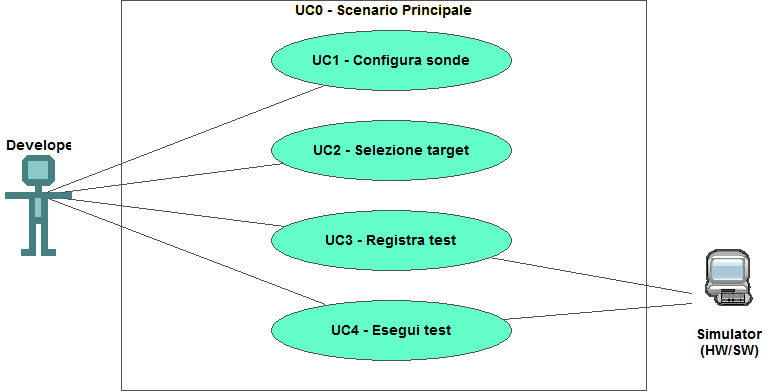
\includegraphics[width=0.9\columnwidth]{usecase/scenario-principale} 
    \caption{Use Case - UC0: Scenario principale}
\end{figure}

\begin{usecase}{0}{Scenario principale}
\usecaseactors{Sviluppatore applicativi}
\usecasepre{Lo sviluppatore è entrato nel plug-in di simulazione all'interno dell'IDE}
\usecasedesc{La finestra di simulazione mette a disposizione i comandi per configurare, registrare o eseguire un test}
\usecasepost{Il sistema è pronto per permettere una nuova interazione}
\label{uc:scenario-principale}
\end{usecase}

\section{Tracciamento dei requisiti}

Da un'attenta analisi dei requisiti e degli use case effettuata sul progetto è stata stilata la tabella che traccia i requisiti in rapporto agli use case.\\
Sono stati individuati diversi tipi di requisiti e si è quindi fatto utilizzo di un codice identificativo per distinguerli.\\
Il codice dei requisiti è così strutturato R(F/Q/V)(N/D/O) dove:
\begin{enumerate}
	\item[R =] requisito
    \item[F =] funzionale
    \item[Q =] qualitativo
    \item[V =] di vincolo
    \item[N =] obbligatorio (necessario)
    \item[D =] desiderabile
    \item[Z =] opzionale
\end{enumerate}
Nelle tabelle \ref{tab:requisiti-funzionali}, \ref{tab:requisiti-qualitativi} e \ref{tab:requisiti-vincolo} sono riassunti i requisiti e il loro tracciamento con gli use case delineati in fase di analisi.

\newpage

\begin{table}%
\caption{Tabella del tracciamento dei requisti funzionali}
\label{tab:requisiti-funzionali}
\begin{tabularx}{\textwidth}{lXl}
\hline\hline
\textbf{Requisito} & \textbf{Descrizione} & \textbf{Use Case}\\
\hline
RFN-1     & L'interfaccia permette di configurare il tipo di sonde del test & UC1 \\
\hline
\end{tabularx}
\end{table}%

\begin{table}%
\caption{Tabella del tracciamento dei requisiti qualitativi}
\label{tab:requisiti-qualitativi}
\begin{tabularx}{\textwidth}{lXl}
\hline\hline
\textbf{Requisito} & \textbf{Descrizione} & \textbf{Use Case}\\
\hline
RQD-1    & Le prestazioni del simulatore hardware deve garantire la giusta esecuzione dei test e non la generazione di falsi negativi & - \\
\hline
\end{tabularx}
\end{table}%

\begin{table}%
\caption{Tabella del tracciamento dei requisiti di vincolo}
\label{tab:requisiti-vincolo}
\begin{tabularx}{\textwidth}{lXl}
\hline\hline
\textbf{Requisito} & \textbf{Descrizione} & \textbf{Use Case}\\
\hline
RVO-1    & La libreria per l'esecuzione dei test automatici deve essere riutilizzabile & - \\
\hline
\end{tabularx}
\end{table}%             % Concept Preview
% !TEX encoding = UTF-8
% !TEX TS-program = pdflatex
% !TEX root = ../tesi.tex
% !TEX spellcheck = it-IT

%**************************************************************
\chapter{Progettazione e codifica}
\label{cap:progettazione-codifica}
%**************************************************************

\intro{Breve introduzione al capitolo}\\

%**************************************************************
\section{Tecnologie e strumenti}
\label{sec:tecnologie-strumenti}

Di seguito viene data una panoramica delle tecnologie e strumenti utilizzati.

\subsection*{Tecnologia 1}
Descrizione Tecnologia 1.

\subsection*{Tecnologia 2}
Descrizione Tecnologia 2

%**************************************************************
\section{Ciclo di vita del software}
\label{sec:ciclo-vita-software}

%**************************************************************
\section{Progettazione}
\label{sec:progettazione}

\subsubsection{Namespace 1} %**************************
Descrizione namespace 1.

\begin{namespacedesc}
    \classdesc{Classe 1}{Descrizione classe 1}
    \classdesc{Classe 2}{Descrizione classe 2}
\end{namespacedesc}


%**************************************************************
\section{Design Pattern utilizzati}

%**************************************************************
\section{Codifica}
             % Product Prototype
% !TEX encoding = UTF-8
% !TEX TS-program = pdflatex
% !TEX root = ../tesi.tex
% !TEX spellcheck = it-IT

%**************************************************************
\chapter{Verifica e validazione}
\label{cap:verifica-validazione}
%**************************************************************             % Product Design Freeze e SOP
% !TEX encoding = UTF-8
% !TEX TS-program = pdflatex
% !TEX root = ../tesi.tex
% !TEX spellcheck = it-IT

%**************************************************************
\chapter{Conclusioni}
\label{cap:conclusioni}
%**************************************************************

%**************************************************************
\section{Consuntivo finale}

%**************************************************************
\section{Raggiungimento degli obiettivi}

%**************************************************************
\section{Conoscenze acquisite}

%**************************************************************
\section{Valutazione personale}
             % Conclusioni
\appendix                               
% !TEX encoding = UTF-8
% !TEX TS-program = pdflatex
% !TEX root = ../tesi.tex
% !TEX spellcheck = it-IT

%**************************************************************
\chapter{Appendice A}
%**************************************************************

\epigraph{Citazione}{Autore della citazione}



             % Appendice A

%**************************************************************
% Materiale finale
%**************************************************************
\backmatter
\printglossaries
% !TEX encoding = UTF-8
% !TEX TS-program = pdflatex
% !TEX root = ../tesi.tex
% !TEX spellcheck = it-IT

%**************************************************************
% Bibliografia
%**************************************************************

\cleardoublepage
\chapter{Bibliografia}

\nocite{*}
%\printbibliography

%\bibbycategory % equivale a dare un \printbibliography per ogni categoria
+\begin{thebibliography}{1}

\bibitem{Zhang-Chen}
Cha Zhang and Tsuhan Chen,
\emph{EFFICIENT FEATURE EXTRACTION FOR 2D/3D OBJECTS IN MESH REPRESENTATION},
Dept. of Electrical and Computer Engineering, Carnegie Mellon University 5000 Forbes 	Avenue, Pittsburgh, PA 15213, USA.

\end{thebibliography}
\end{document}